\documentclass[10pt,twocolumn]{article}

% ── Packages ──────────────────────────────────────────────────────────
\usepackage[utf8]{inputenc}
\usepackage[T1]{fontenc}
\usepackage[margin=2cm]{geometry}
\usepackage{amsmath,amssymb,amsfonts}
\usepackage{graphicx}
\usepackage{booktabs}
\usepackage{multirow}
\usepackage{hyperref}
\usepackage{xcolor}
\usepackage{caption}
\usepackage{subcaption}
\usepackage[numbers,sort&compress]{natbib}
\usepackage{algorithm}
\usepackage{algorithmic}
\usepackage{enumitem}
\usepackage{microtype}

\graphicspath{{figures/}}

\hypersetup{
  colorlinks=true,
  linkcolor=blue!60!black,
  citecolor=green!50!black,
  urlcolor=blue!70!black
}

% ── Compact spacing ──────────────────────────────────────────────────
\setlength{\parskip}{0.4em}
\setlength{\abovecaptionskip}{6pt}
\setlength{\belowcaptionskip}{2pt}

% ── Title ────────────────────────────────────────────────────────────
\title{%
  \textbf{How Fragile Are Your Explanations?}\\[4pt]
  Measuring the Stability of SHAP Attributions\\
  Under Distributional Shift%
}

\author{
  Anonymous Author(s)\\
  \textit{Department of Applied Mathematics}\\
  \texttt{anonymous@university.edu}
}

\date{}

% ═════════════════════════════════════════════════════════════════════
\begin{document}
\maketitle

% ── Abstract ─────────────────────────────────────────────────────────
\begin{abstract}
SHAP is one of the most popular methods for explaining machine
learning predictions, but there is surprisingly little work on what
happens to those explanations when the data is noisy or corrupted.
In this paper, we run a set of experiments to measure how stable
SHAP explanations are when the input data is perturbed in three
ways: Gaussian noise added to features, random corruption of
training labels, and dropout of feature values. We test across
three UCI/Kaggle classification datasets and four model types
(XGBoost, Logistic Regression, Decision Tree, and Explainable
Boosting Machine), running over 6{,}000 experiments in total.
We use a set of stability metrics grounded in Lipschitz-style
sensitivity analysis and rank correlation measures.

Our main results are: (1)~label corruption has a much larger effect
on explanations than the other two perturbation types---Spearman
rank correlation between original and perturbed SHAP rankings
drops to $\rho = 0.28$ under just 5\% label noise, while Gaussian
noise leaves it above 0.95; (2)~rank stability and magnitude
stability turn out to be quite different things---a model can keep
the same feature ranking while its actual SHAP values shift by
$7.7\times$ the input perturbation; (3)~the Explainable Boosting
Machine is the most stable model overall; (4)~Decision Trees,
often called ``inherently interpretable,'' actually produce the
least stable explanations; and (5)~under enough label corruption,
SHAP fidelity can go negative, meaning the explanations are worse
than useless. We also give some practical recommendations based
on these findings.
\end{abstract}

\textbf{Keywords:} Explainability, SHAP, Stability, Distributional
Shift, Interpretable Machine Learning

% ═════════════════════════════════════════════════════════════════════
\section{Introduction}\label{sec:intro}

In many applied settings---healthcare, finance, credit
scoring---people need to understand \emph{why} a model makes the
predictions it does, not just what those predictions are.
SHAP~\cite{lundberg2017unified} has become one of the standard tools
for this. It assigns each input feature a contribution score based
on Shapley values from cooperative game theory, and it has nice
theoretical properties: the attributions are locally faithful and
add up to the model's prediction.

But there is a practical question that does not seem to get much
attention: \emph{how much do these explanations change when the
data is a bit noisy?} In real-world applications, data is rarely
clean. Measurements have noise, labels sometimes get recorded
wrong, and features can be missing. If a small amount of noise
completely reshuffles which features SHAP says are important, then
those explanations are not very useful in practice.

Some prior work has looked at related questions.
Alvarez-Melis and Jaakkola~\cite{alvarez2018robustness} studied
local Lipschitz continuity of explanations, and
Slack~et~al.~\cite{slack2020fooling} showed that SHAP and LIME can
be fooled by adversarial attacks. But these studies tend to look at
one perturbation type at a time, or one model at a time, and they
do not really compare across multiple dimensions of stability
(does the ranking change? by how much do the values shift? is the
explanation still faithful to the model?).

In this paper, we try to address this gap by running a fairly
comprehensive set of experiments. Specifically, we:
\begin{enumerate}[leftmargin=*,topsep=2pt,itemsep=1pt]
  \item Define a set of stability metrics that capture rank
    stability, magnitude sensitivity, and faithfulness. For
    training-time perturbations where the inputs do not change
    (only the labels do), we define a model-space Lipschitz ratio
    that measures how SHAP values respond to changes in the model
    parameters.
  \item Run experiments across 3 datasets, 4 models, 3 perturbation
    types, 3 intensity levels, and 5 random seeds (over 6{,}000
    runs total), with statistical testing to check significance.
  \item Report five findings that we think are interesting, a few
    of which go against common assumptions---for instance, that
    Decision Trees give more ``trustworthy'' explanations than
    black-box models.
  \item Provide some practical guidelines for people who want to
    use SHAP in settings where data quality is uncertain.
\end{enumerate}

% ═════════════════════════════════════════════════════════════════════
\section{Related Work}\label{sec:related}

\subsection{Post-Hoc Explanation Methods}

SHAP~\cite{lundberg2017unified} uses Shapley values from game theory
to explain individual predictions. For tree-based models, the
TreeExplainer algorithm computes these values exactly in polynomial
time, which is nice because it avoids the approximation errors that
come with sampling-based methods.
LIME~\cite{ribeiro2016why} takes a different approach, fitting a
sparse linear model around each prediction. Both methods are mainly
evaluated on clean, static datasets in the original papers.

\subsection{Explanation Robustness}

Alvarez-Melis and Jaakkola~\cite{alvarez2018robustness} proposed
local Lipschitz continuity as a way to measure how sensitive
explanations are to small input changes, and found that many methods
are quite sensitive. Slack~et~al.~\cite{slack2020fooling} went further
and showed that SHAP and LIME can be deliberately fooled by an
adversary. Dombrowski~et~al.~\cite{dombrowski2019explanations} showed
a related result for gradient-based explanations on neural networks.

\subsection{What Is Missing}

A recent large-scale comparison of 16 interpretable
methods~\cite{comparative2026} tested accuracy on 216 datasets,
but stability under perturbation was not part of the evaluation. A
study of sparse Vision Transformers~\cite{sparse2026vit} found that
making a model structurally simpler does not necessarily make its
explanations more stable---sparsity ``redistributes rather than
isolates computation.'' The Schmidt Sciences 2026
RFP~\cite{schmidt2026rfp} specifically asks for explanation methods
that work ``beyond academic benchmarks.'' All of this suggests that
there is room for a study that looks at explanation stability in a
more structured way: across different kinds of perturbations,
different model types, and different notions of what ``stable''
means.

% ═════════════════════════════════════════════════════════════════════
\section{Methodology}\label{sec:method}

\subsection{Stability Metrics}\label{sec:metrics}

We wanted to measure stability along several dimensions, since a
single number does not tell the full story. We settled on three
categories.

\paragraph{Rank stability.}
The most basic question is whether the ordering of features by
importance stays the same. We measure this with \emph{Spearman rank
correlation} ($\rho_s$) between the original and perturbed SHAP
rankings. A value of $\rho_s > 0.8$ indicates the rankings are
largely preserved. We also use \emph{Top-$k$ Jaccard similarity}
to check whether the set of most important features is preserved:
\begin{equation}\label{eq:jaccard}
  J_k = \frac{|S_k \cap S'_k|}{|S_k \cup S'_k|}, \quad k \in \{3,5\}.
\end{equation}

\paragraph{Magnitude stability.}
Even if the ranking is preserved, the actual SHAP values might shift
a lot. We measure this using a Lipschitz-style ratio. The
\emph{input-space Lipschitz ratio} is:
\begin{equation}\label{eq:lipschitz}
  L = \frac{\|\mathrm{SHAP}(\mathbf{x}') - \mathrm{SHAP}(\mathbf{x})\|_2}
           {\|\mathbf{x}' - \mathbf{x}\|_2},
\end{equation}
which tells us how much the SHAP values change per unit of input
change. This works for Gaussian noise and feature dropout, where
the input actually changes. But for label flip, the inputs stay the
same and only the model changes (because it gets retrained). So we
define a \emph{model-space Lipschitz ratio}:
\begin{equation}\label{eq:model_lipschitz}
  L_\theta = \frac{\|\Delta\mathrm{SHAP}\|_2}
                   {\|\Delta\boldsymbol\theta\|_2},
\end{equation}
where $\boldsymbol\theta$ represents the model parameters (e.g.,
coefficients for Logistic Regression, feature importances for
tree-based models).

\paragraph{Faithfulness.}
We also want to know if the explanation is still \emph{accurate} as
a description of the model. \emph{Surrogate fidelity} checks how
well the SHAP additive decomposition reproduces the model's
predictions:
\begin{equation}\label{eq:fidelity}
  \text{Fidelity} = 1 - \frac{\text{MAE}(f, g)}
                              {\text{MAE}(f, \bar{y})},
\end{equation}
where $g(\mathbf{x}) = \mathbb{E}[f(\mathbf{x})] + \sum_j
\phi_j(\mathbf{x})$ is the SHAP reconstruction. If this goes
negative, the SHAP explanation does worse than just predicting the
mean---it is actively misleading. We also compute a
\emph{perturbation faithfulness ratio} $\text{FR}_k$: the ratio of
the prediction drop when we mask the top-$k$ SHAP features vs.\
the bottom-$k$. A high ratio confirms SHAP is pointing at the
right features.

\subsection{Perturbation Protocol}\label{sec:perturbation}

We apply three types of perturbation, each meant to model a
different kind of data quality problem:
\begin{enumerate}[leftmargin=*,topsep=2pt,itemsep=1pt]
  \item \textbf{Gaussian noise} (applied at test time):
    $\mathbf{x}' = \mathbf{x} + \boldsymbol\varepsilon$,
    $\boldsymbol\varepsilon \sim \mathcal{N}(0,\sigma^2\mathbf{I})$,
    with $\sigma \in \{0.05, 0.10, 0.15\}$. This models sensor
    noise or measurement error. The model is not retrained.
  \item \textbf{Label flip} (applied at training time): randomly
    flip $y_{\text{train}}$ labels at rates $\{5\%, 10\%, 15\%\}$.
    This models annotation errors. The model \emph{is} retrained
    on the corrupted labels.
  \item \textbf{Feature dropout} (applied at test time): set
    feature values to zero with probability
    $\{0.05, 0.10, 0.15\}$. This models missing data. The model is
    not retrained.
\end{enumerate}

\subsection{Datasets}\label{sec:datasets}

We use three standard classification datasets (Table~\ref{tab:datasets}).
These are small-to-medium in size, which let us run many
experimental configurations. All features are standardized to
zero mean and unit variance. We use 80/20 stratified train-test
splits and repeat each experiment with 5 different random seeds.

\begin{table}[t]
\centering
\caption{Dataset summary.}\label{tab:datasets}
\small
\begin{tabular}{@{}lcccl@{}}
\toprule
\textbf{Dataset} & $n$ & $p$ & \textbf{Domain} & \textbf{Source} \\
\midrule
Heart Disease~\cite{uci_heart}        & 297  & 13 & Cardiology     & UCI    \\
Pima Diabetes~\cite{smith1988pima}     & 768  &  8 & Endocrinology  & Kaggle \\
Breast Cancer~\cite{wolberg1995breast} & 569  & 30 & Oncology       & UCI    \\
\bottomrule
\end{tabular}
\end{table}

\subsection{Models}\label{sec:models}

We pick two ``black-box'' models and two ``interpretable'' models
(Table~\ref{tab:models}). This lets us compare whether model
transparency actually helps with explanation stability.

\begin{table}[t]
\centering
\caption{Model configurations.}\label{tab:models}
\small
\begin{tabular}{@{}llll@{}}
\toprule
\textbf{Model} & \textbf{Type} & \textbf{SHAP Method} & \textbf{Key Params} \\
\midrule
XGBoost~\cite{chen2016xgboost}     & Black-box  & TreeExplainer   & 100 trees, depth~6  \\
Logistic Reg.                       & Black-box  & LinearExplainer & L2, $C\!=\!1.0$     \\
Decision Tree                       & Interpretable & TreeExplainer & depth~5, leaf~10    \\
EBM~\cite{nori2019interpretml}      & Interpretable & Native local  & 256 bins, 10 int.   \\
\bottomrule
\end{tabular}
\end{table}

% ═════════════════════════════════════════════════════════════════════
\section{Results}\label{sec:results}

We ran 6{,}147 experiment configurations in total. Below, we
organize the results around five main observations.

\subsection{Label Corruption Dominates Everything Else}\label{sec:f1}

This was the clearest result. Under Gaussian noise and feature
dropout, Spearman $\rho$ stays above 0.95 for every model-dataset
pair we tested. But under label flip, it drops sharply---down to
0.28 for Breast Cancer with Logistic Regression
(Table~\ref{tab:perturbation}).

The difference is statistically significant in all cases. We ran
Mann--Whitney $U$ tests comparing label flip against the other two
perturbation types, and all six comparisons gave $p < 0.001$
with Cohen's $d$ ranging from 1.73 to 8.70.

\begin{table}[t]
\centering
\caption{Mean Spearman $\rho$ by perturbation type, averaged across
  all four models and perturbation levels.}\label{tab:perturbation}
\small
\begin{tabular}{@{}lccc@{}}
\toprule
\textbf{Dataset}  & \textbf{Gaussian} & \textbf{Dropout} & \textbf{Label Flip} \\
\midrule
Heart Disease      & $0.987 \pm 0.021$ & $0.993 \pm 0.005$ & $0.754 \pm 0.104$ \\
Pima Diabetes      & $0.993 \pm 0.009$ & $0.991 \pm 0.012$ & $0.884 \pm 0.071$ \\
Breast Cancer      & $0.999 \pm 0.001$ & $0.996 \pm 0.003$ & $0.425 \pm 0.164$ \\
\bottomrule
\end{tabular}
\end{table}

\begin{figure}[t]
\centering
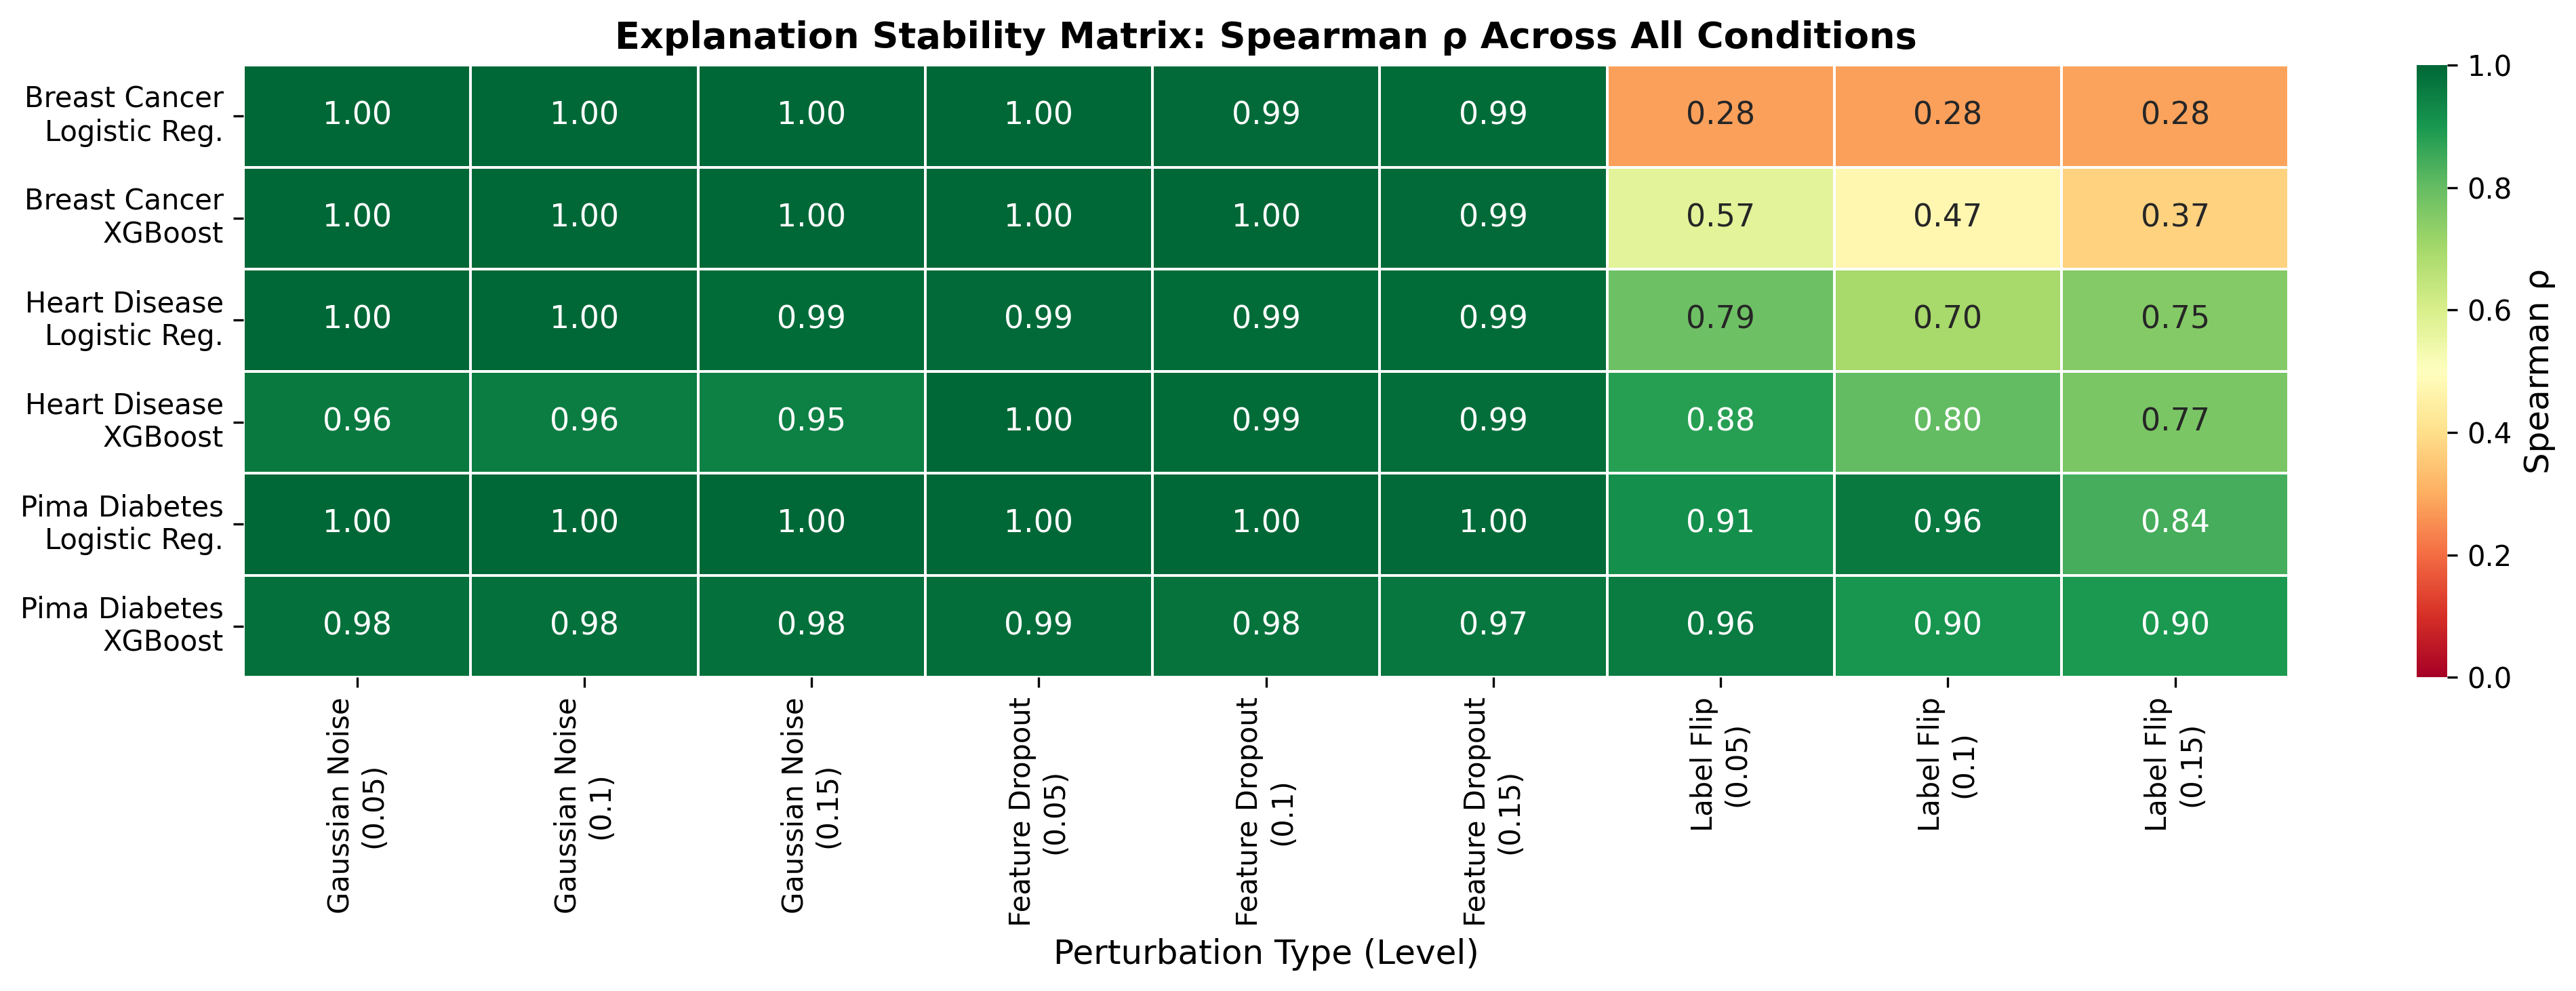
\includegraphics[width=\linewidth]{stability_heatmap.png}
\caption{Stability heatmap across all conditions. Green means stable
  ($\rho \approx 1$); red means unstable. The label flip row stands
  out clearly.}\label{fig:heatmap}
\end{figure}

\begin{figure}[t]
\centering
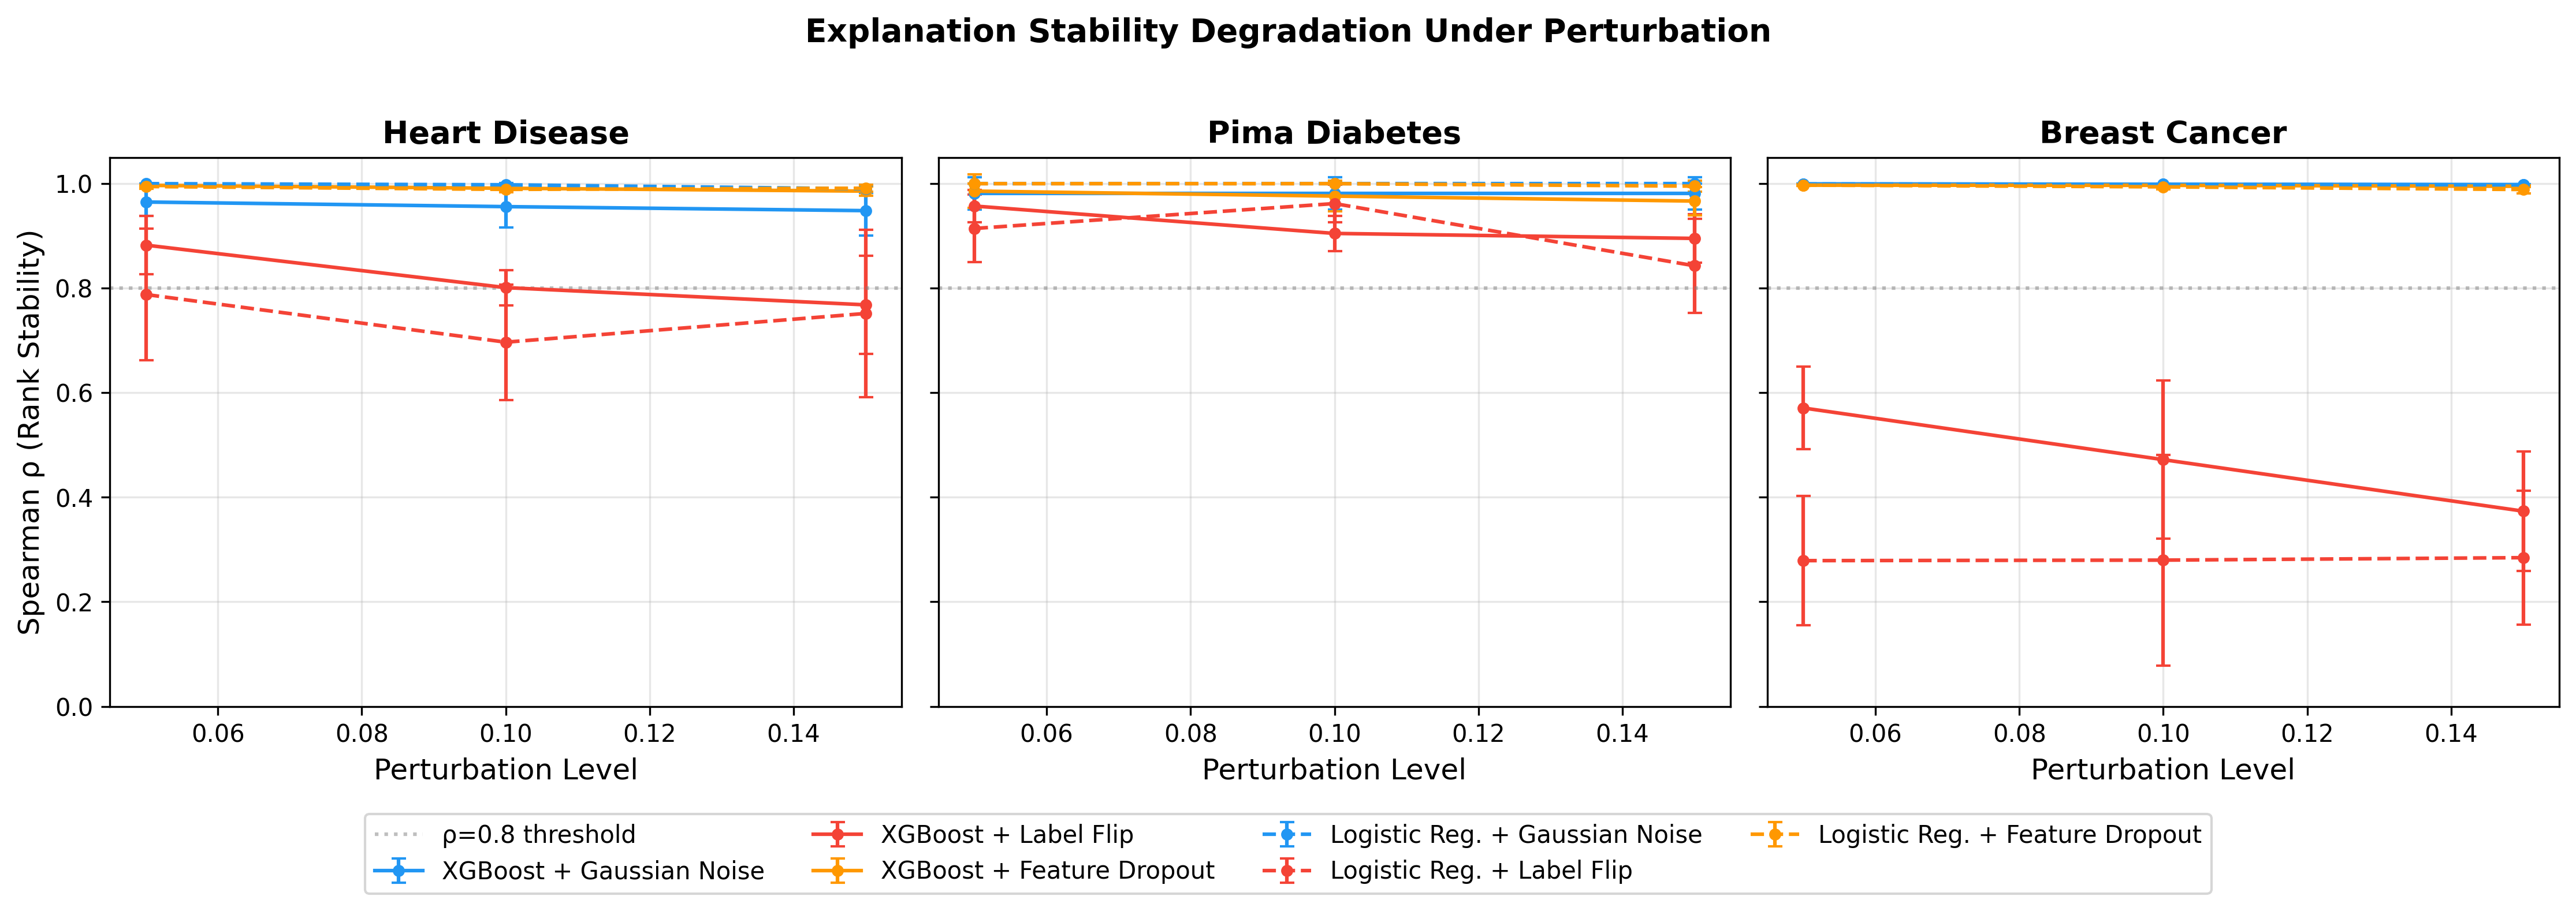
\includegraphics[width=\linewidth]{degradation_curves.png}
\caption{How $\rho$ degrades as perturbation intensity increases.
  Label flip (red) drops steeply; the other two stay
  flat.}\label{fig:degradation}
\end{figure}

\subsection{Rank Stability and Magnitude Stability Are Not the
            Same Thing}\label{sec:f2}

This was somewhat surprising to us. XGBoost on Heart Disease has
$\rho = 0.96$ under 5\% Gaussian noise, which looks very stable if
you only look at rankings. But its Lipschitz ratio is $L = 7.67$,
meaning the SHAP values move $7.7\times$ faster than the input
perturbation in $\ell_2$ norm. The ranking stays the same, but the
actual numbers change a lot.

Logistic Regression, by contrast, has $L < 0.67$ across all
conditions---it is stable in both senses. This distinction matters
because in some applications (e.g., regulatory compliance) people
care about the exact SHAP values, not just which feature is on top.

\begin{figure}[t]
\centering
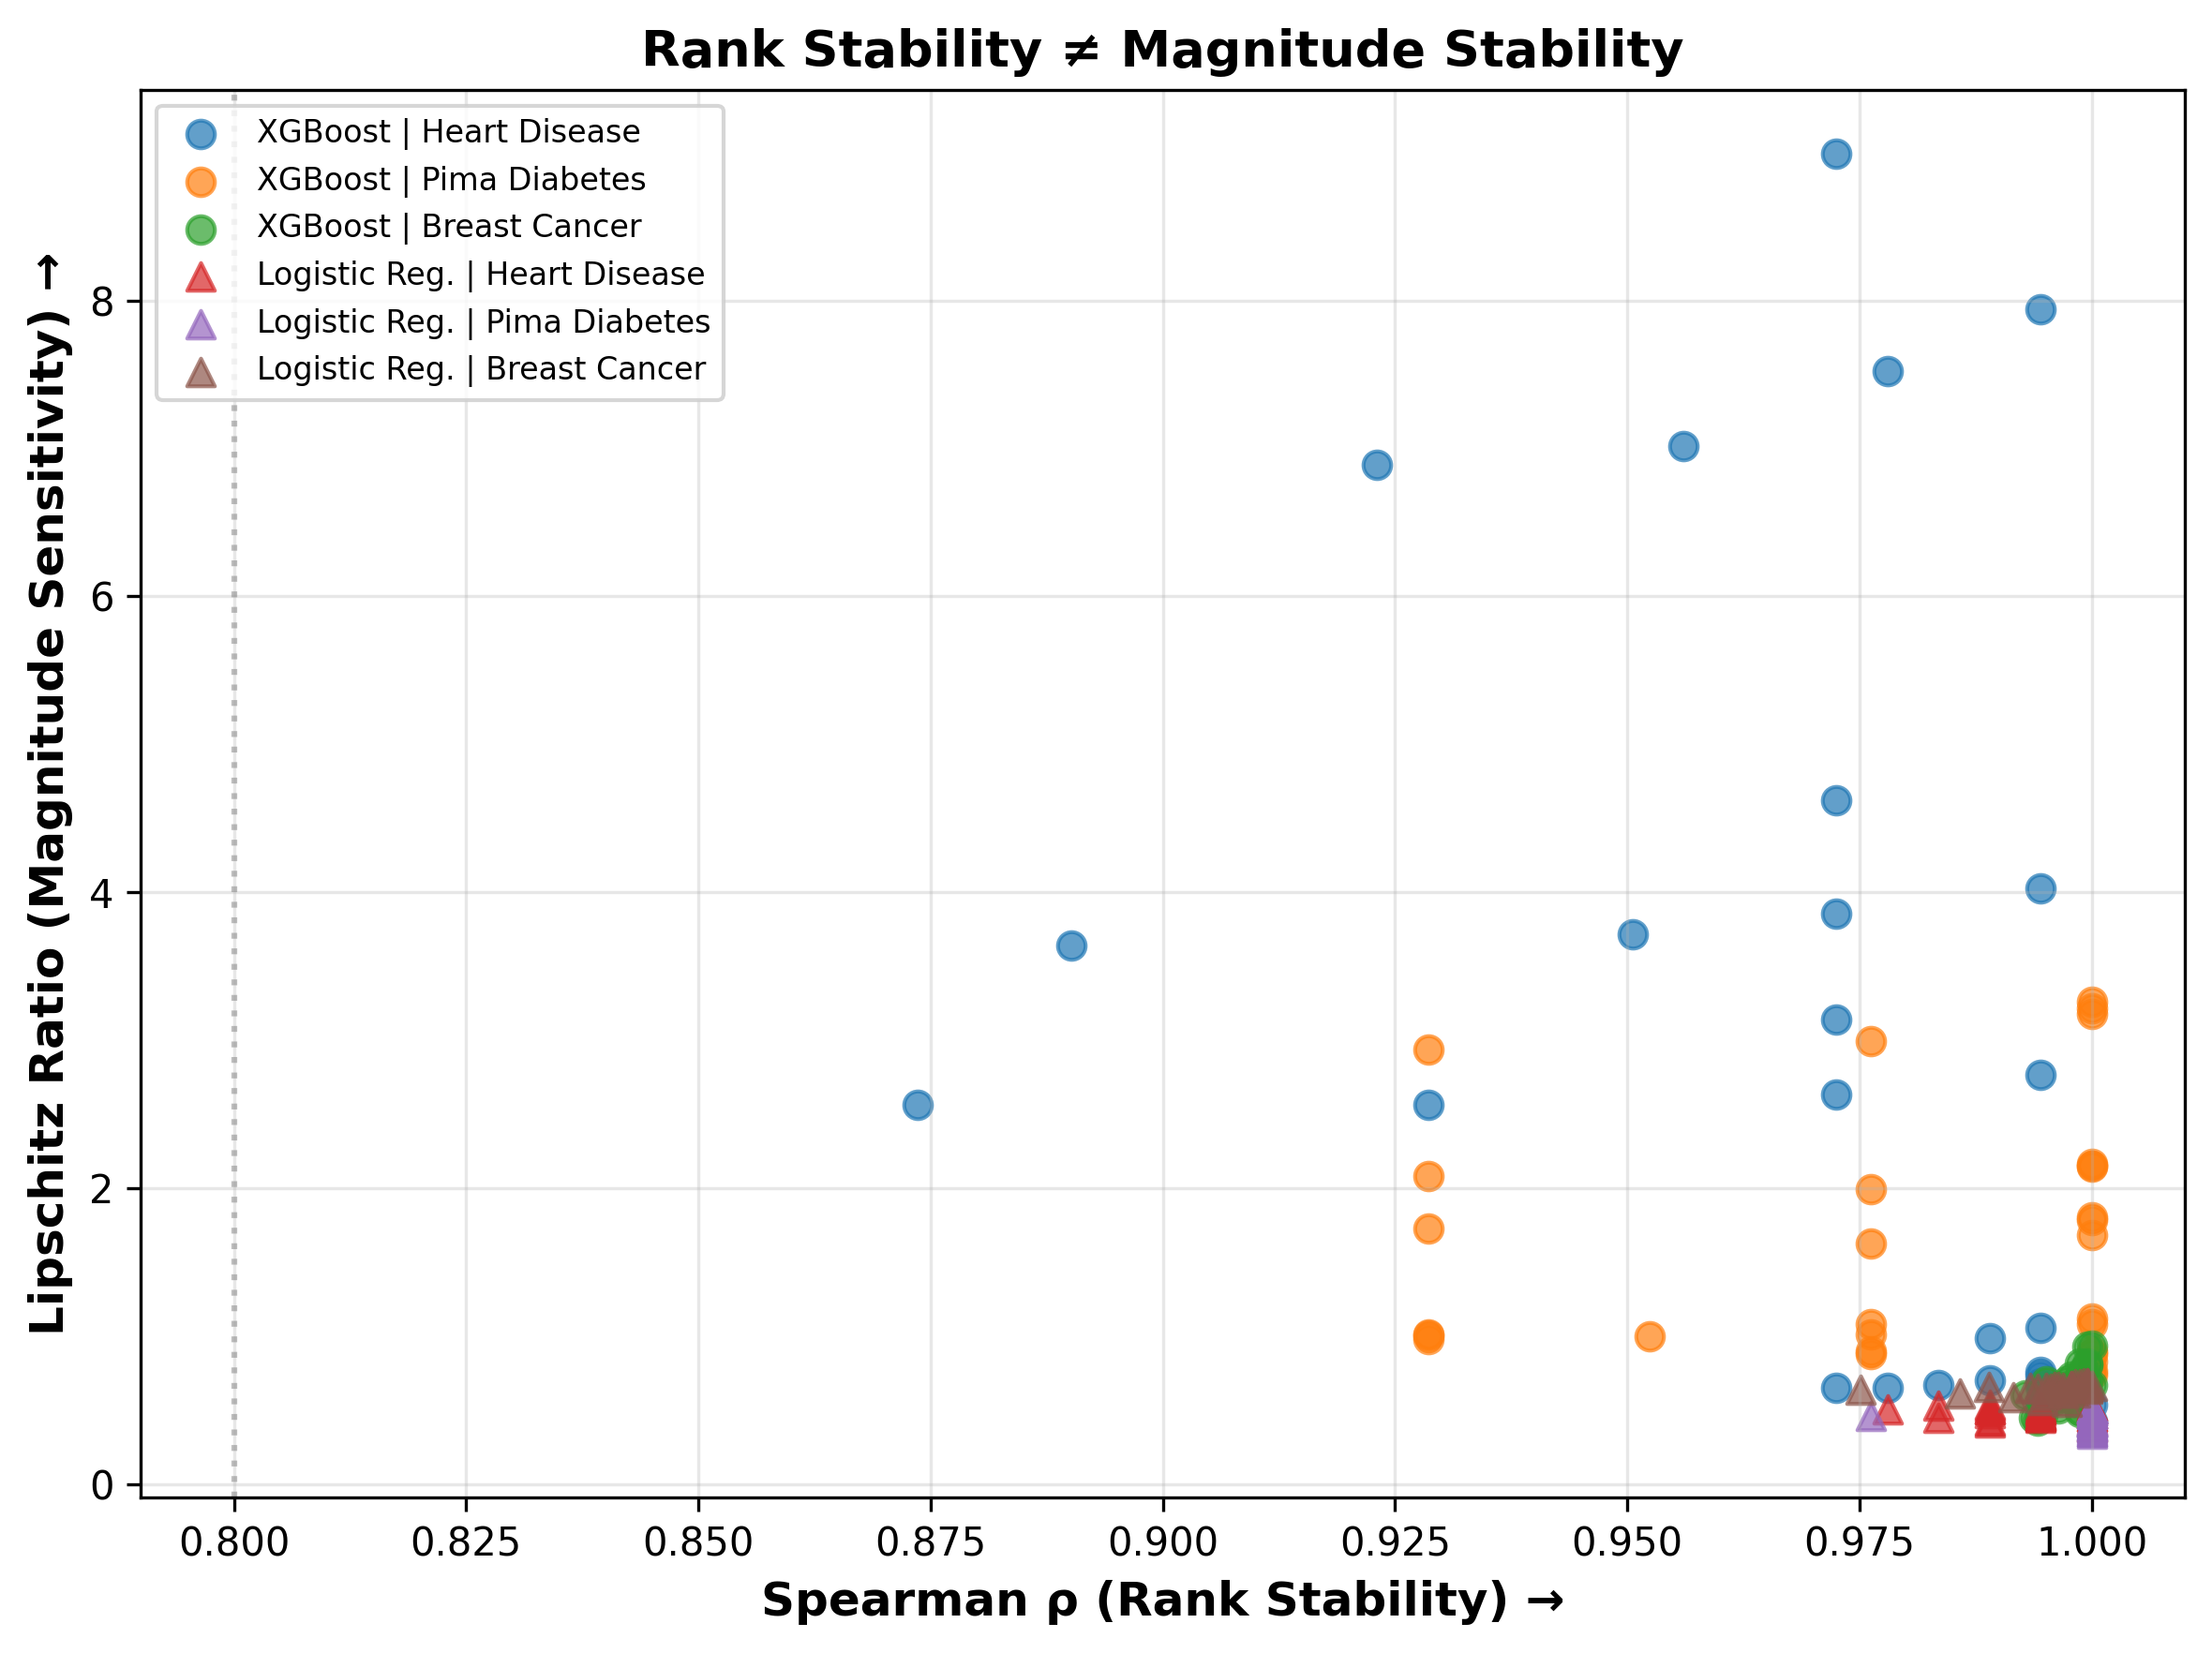
\includegraphics[width=0.9\linewidth]{rank_vs_magnitude.png}
\caption{Rank stability ($\rho$) plotted against magnitude
  sensitivity ($L$). Points in the upper-right corner are
  rank-stable but magnitude-unstable.}\label{fig:rank_mag}
\end{figure}

\begin{figure}[t]
\centering
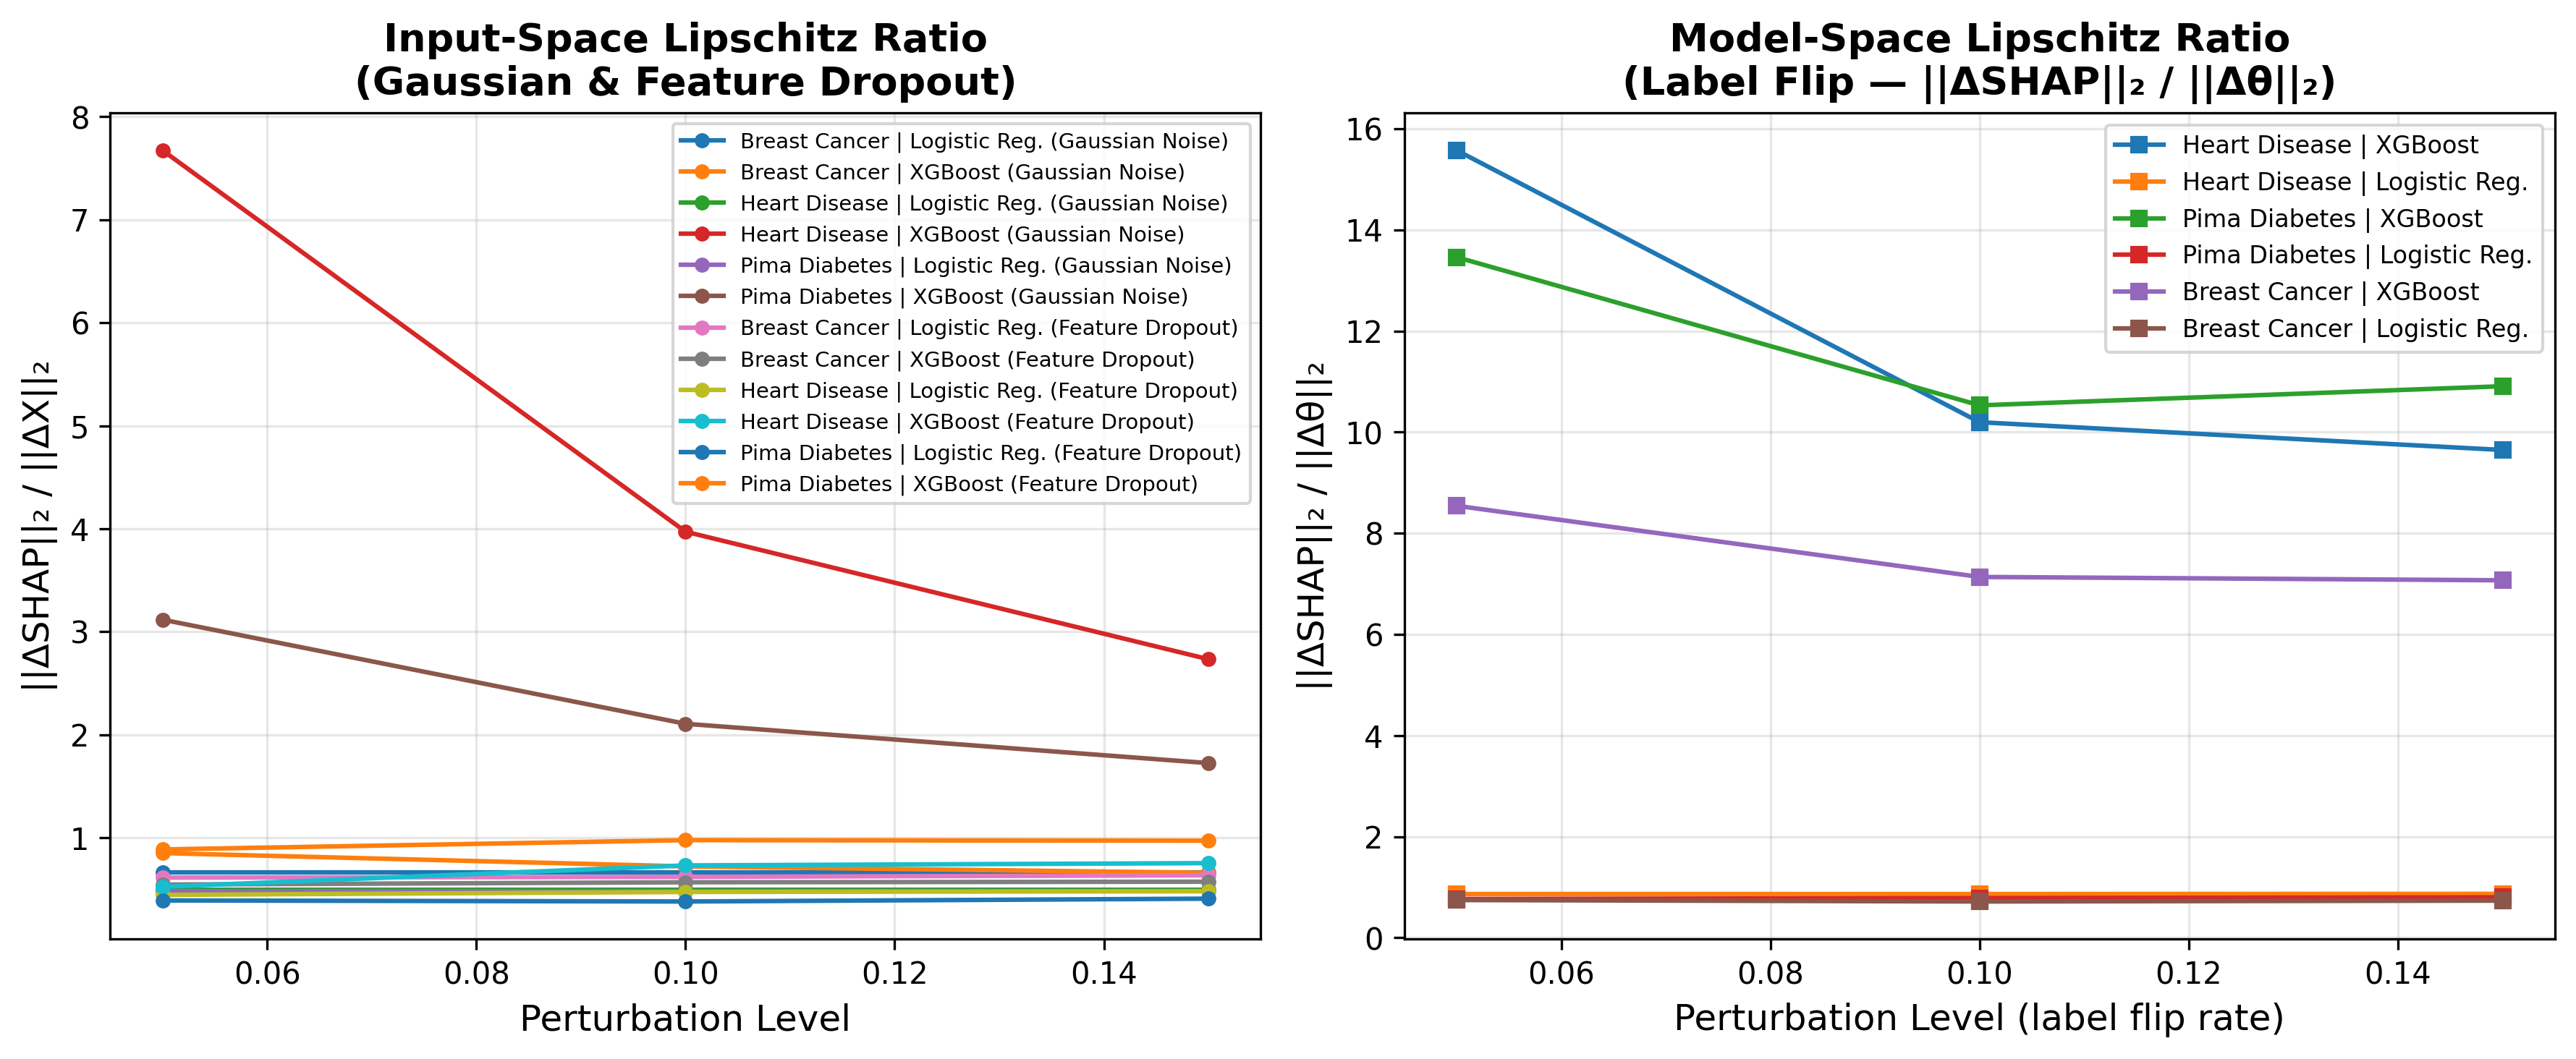
\includegraphics[width=\linewidth]{lipschitz_comparison.png}
\caption{Lipschitz ratios across models. Left: input-space (Gaussian
  noise, feature dropout). Right: model-space (label
  flip).}\label{fig:lipschitz}
\end{figure}

\subsection{EBM Gives the Most Stable Explanations}\label{sec:f3}

Among the four models, the Explainable Boosting
Machine~\cite{nori2019interpretml} tends to come out on top for
stability under label flip (Table~\ref{tab:model_stability}). On
Breast Cancer, which has 30 features, EBM's $\rho = 0.608$ is about
$2.2\times$ higher than Logistic Regression's $0.281$.

We think this is because of EBM's additive structure: it models each
feature independently as $f(\mathbf{x}) = \sum_j h_j(x_j)$, so
corrupted labels cannot easily cause one feature's contribution to
``spill over'' into another.

\begin{table}[t]
\centering
\caption{Mean Spearman $\rho$ under label flip, by
  model.}\label{tab:model_stability}
\small
\begin{tabular}{@{}lcccc@{}}
\toprule
\textbf{Dataset} & \textbf{EBM} & \textbf{XGBoost} & \textbf{LogReg} & \textbf{DecTree} \\
\midrule
Heart     & 0.798 & \textbf{0.817} & 0.745 & 0.656 \\
Diabetes  & \textbf{0.919} & 0.919 & 0.906 & 0.792 \\
Breast Ca.& \textbf{0.608} & 0.472 & 0.281 & 0.341 \\
\bottomrule
\end{tabular}
\end{table}

\begin{figure}[t]
\centering
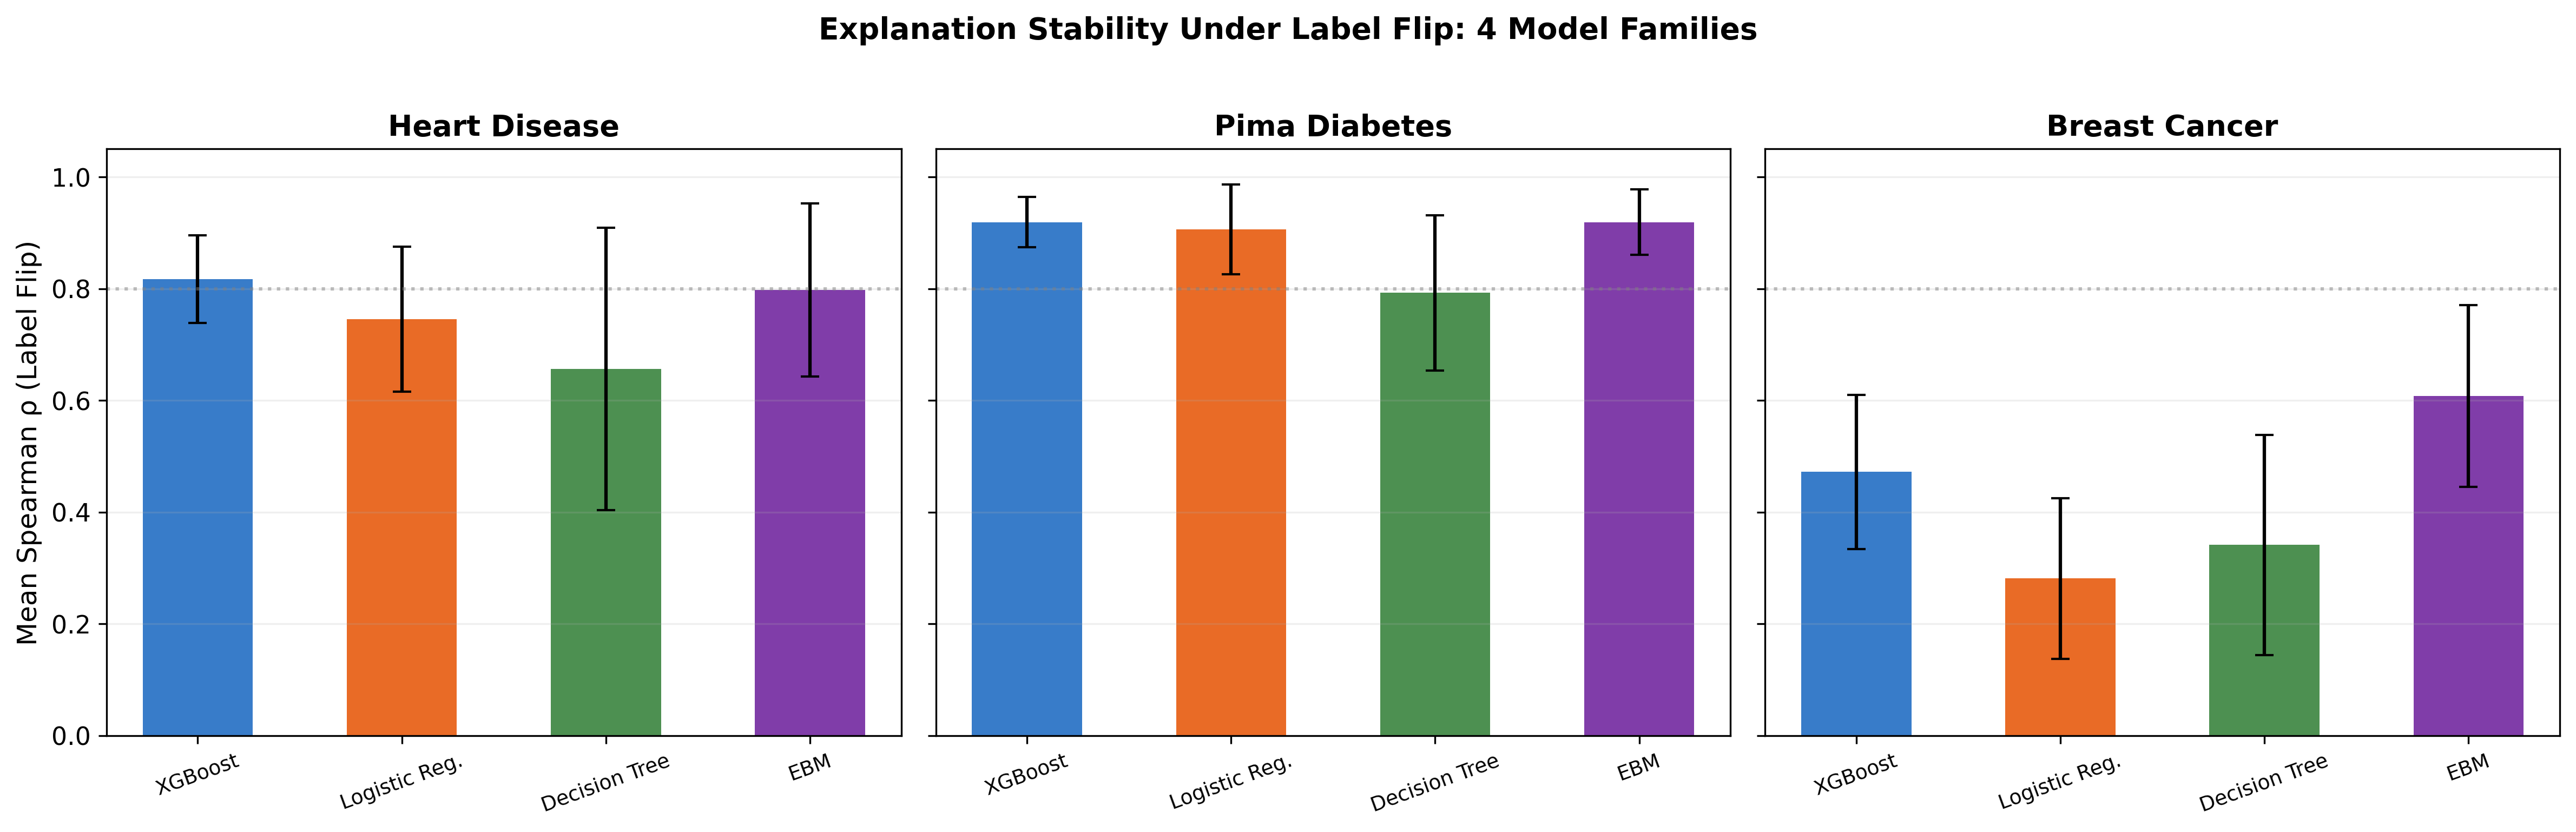
\includegraphics[width=\linewidth]{model_comparison_bars.png}
\caption{Stability (mean $\rho$) under label flip, grouped by
  model.}\label{fig:bars}
\end{figure}

\begin{figure}[t]
\centering
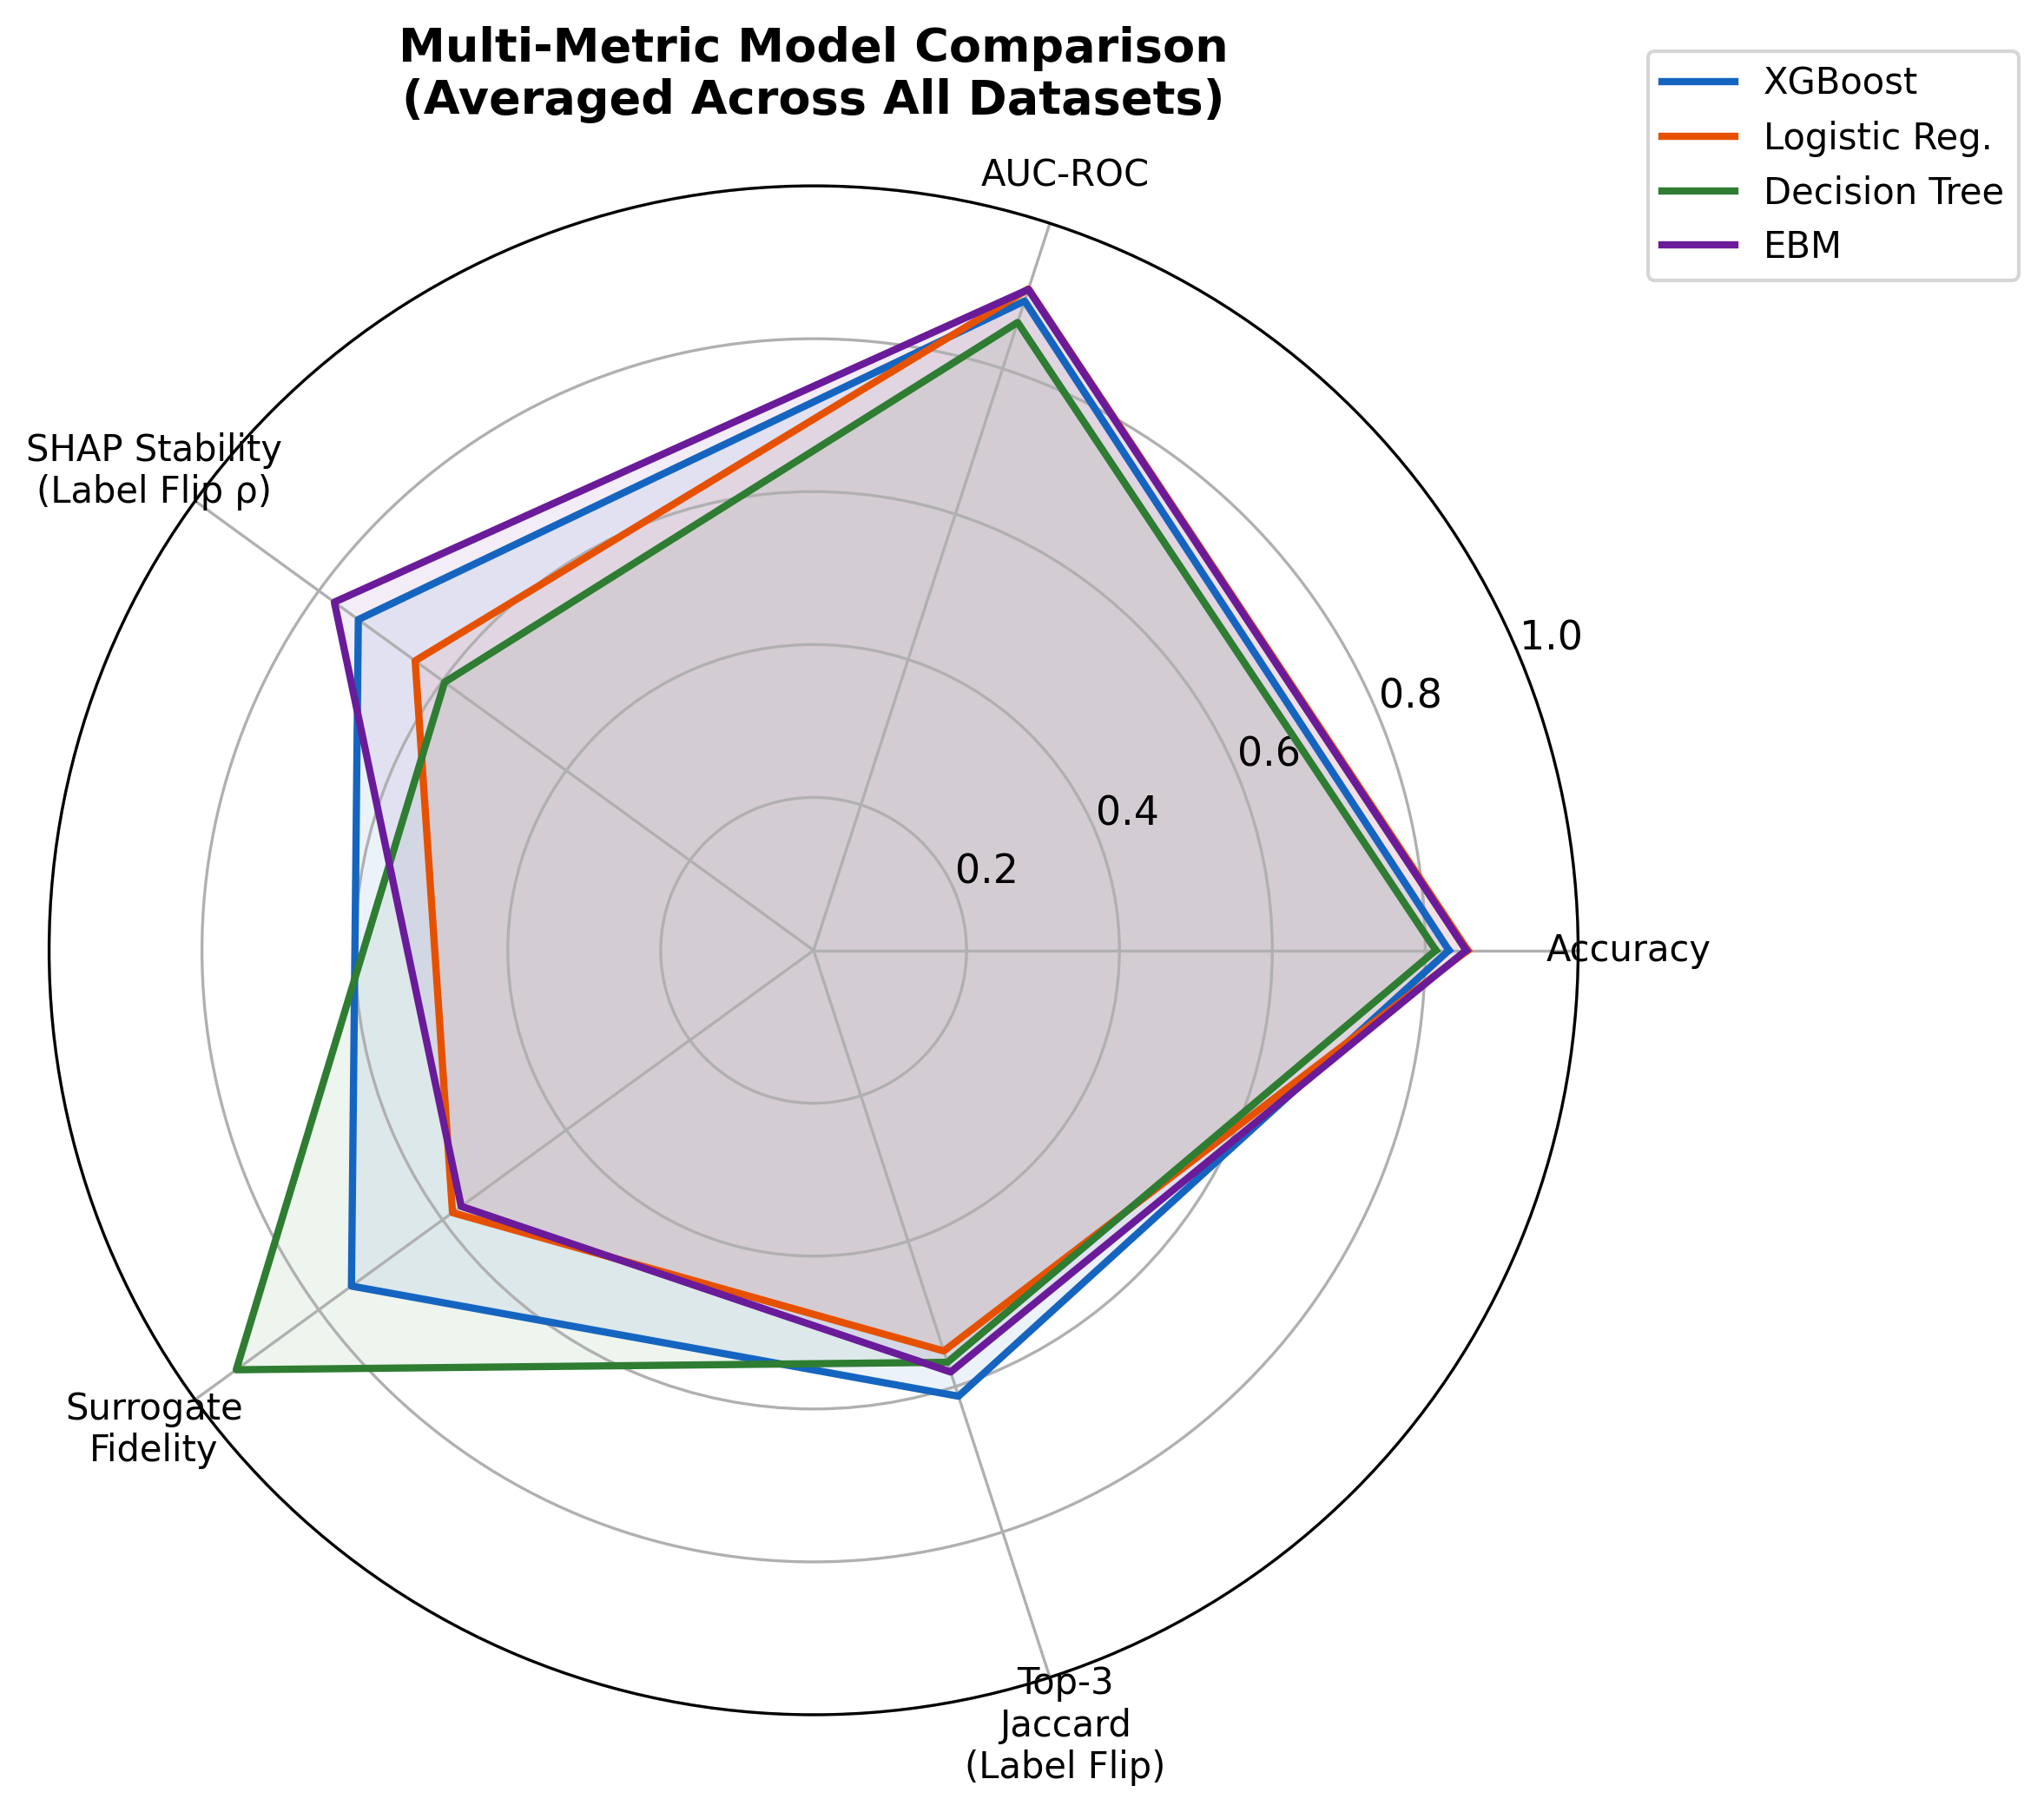
\includegraphics[width=0.9\linewidth]{radar_comparison.png}
\caption{Radar chart comparing all four models across accuracy,
  AUC-ROC, SHAP stability, fidelity, and Top-3 Jaccard under
  label flip. EBM has the most balanced
  profile.}\label{fig:radar}
\end{figure}

\subsection{Decision Trees Are Less Stable Than You Would
            Expect}\label{sec:f4}

This was probably the most counterintuitive result. Decision Trees
are often described as ``inherently interpretable,'' which might
lead you to think their explanations are also stable. But they are
actually among the worst: $\rho = 0.341$ on Breast Cancer and
$0.656$ on Heart Disease under label flip.

The reason, we believe, is structural. A Decision Tree is
piecewise-constant: each leaf assigns a fixed value, and the
boundaries between regions are determined by split points. A small
change in training labels can move a split point, which restructures
the entire tree topology and redistributes feature importance in a
way that is hard to predict.

\begin{figure}[t]
\centering
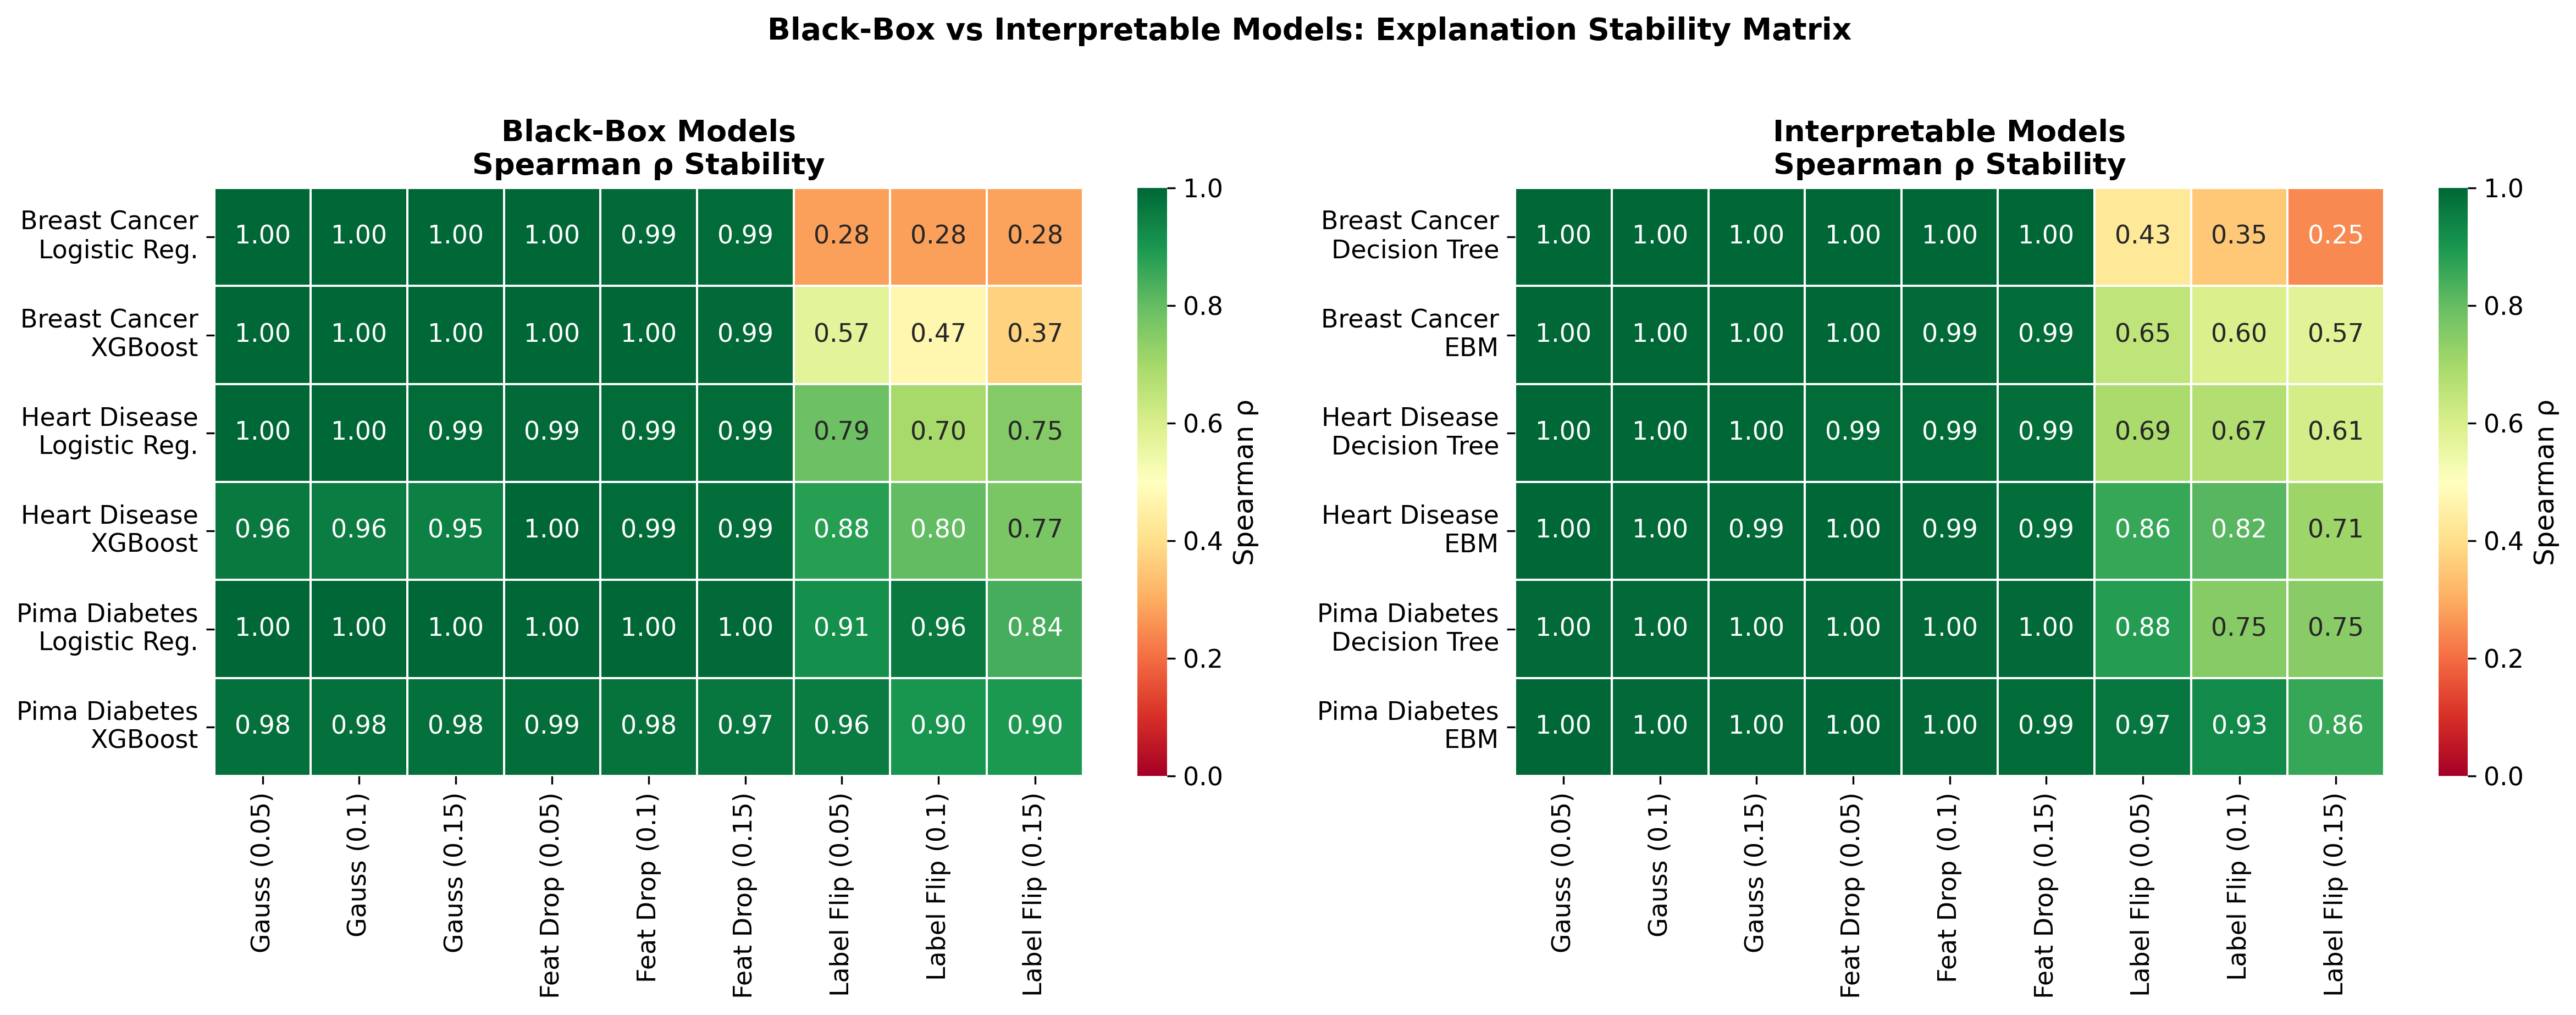
\includegraphics[width=\linewidth]{blackbox_vs_interpretable_heatmap.png}
\caption{Black-box vs.\ interpretable model stability. Decision
  Trees (right panel, lower rows) show as much or more instability
  as the black-box models under label flip.}\label{fig:bb_vs_interp}
\end{figure}

\subsection{SHAP Fidelity Can Go Negative}\label{sec:f5}

Under 15\% label flip, surrogate fidelity drops to $-0.50$ for
Pima Diabetes with Logistic Regression. Negative fidelity means
the SHAP additive decomposition does worse at predicting the
model's output than just guessing the average---the explanation is
not just noisy, it is actively wrong.

All six faithfulness tests under label flip are significant at
$p < 0.01$ (Mann--Whitney $U$, Cohen's $d$ between 1.81 and 2.35).

\begin{figure}[t]
\centering
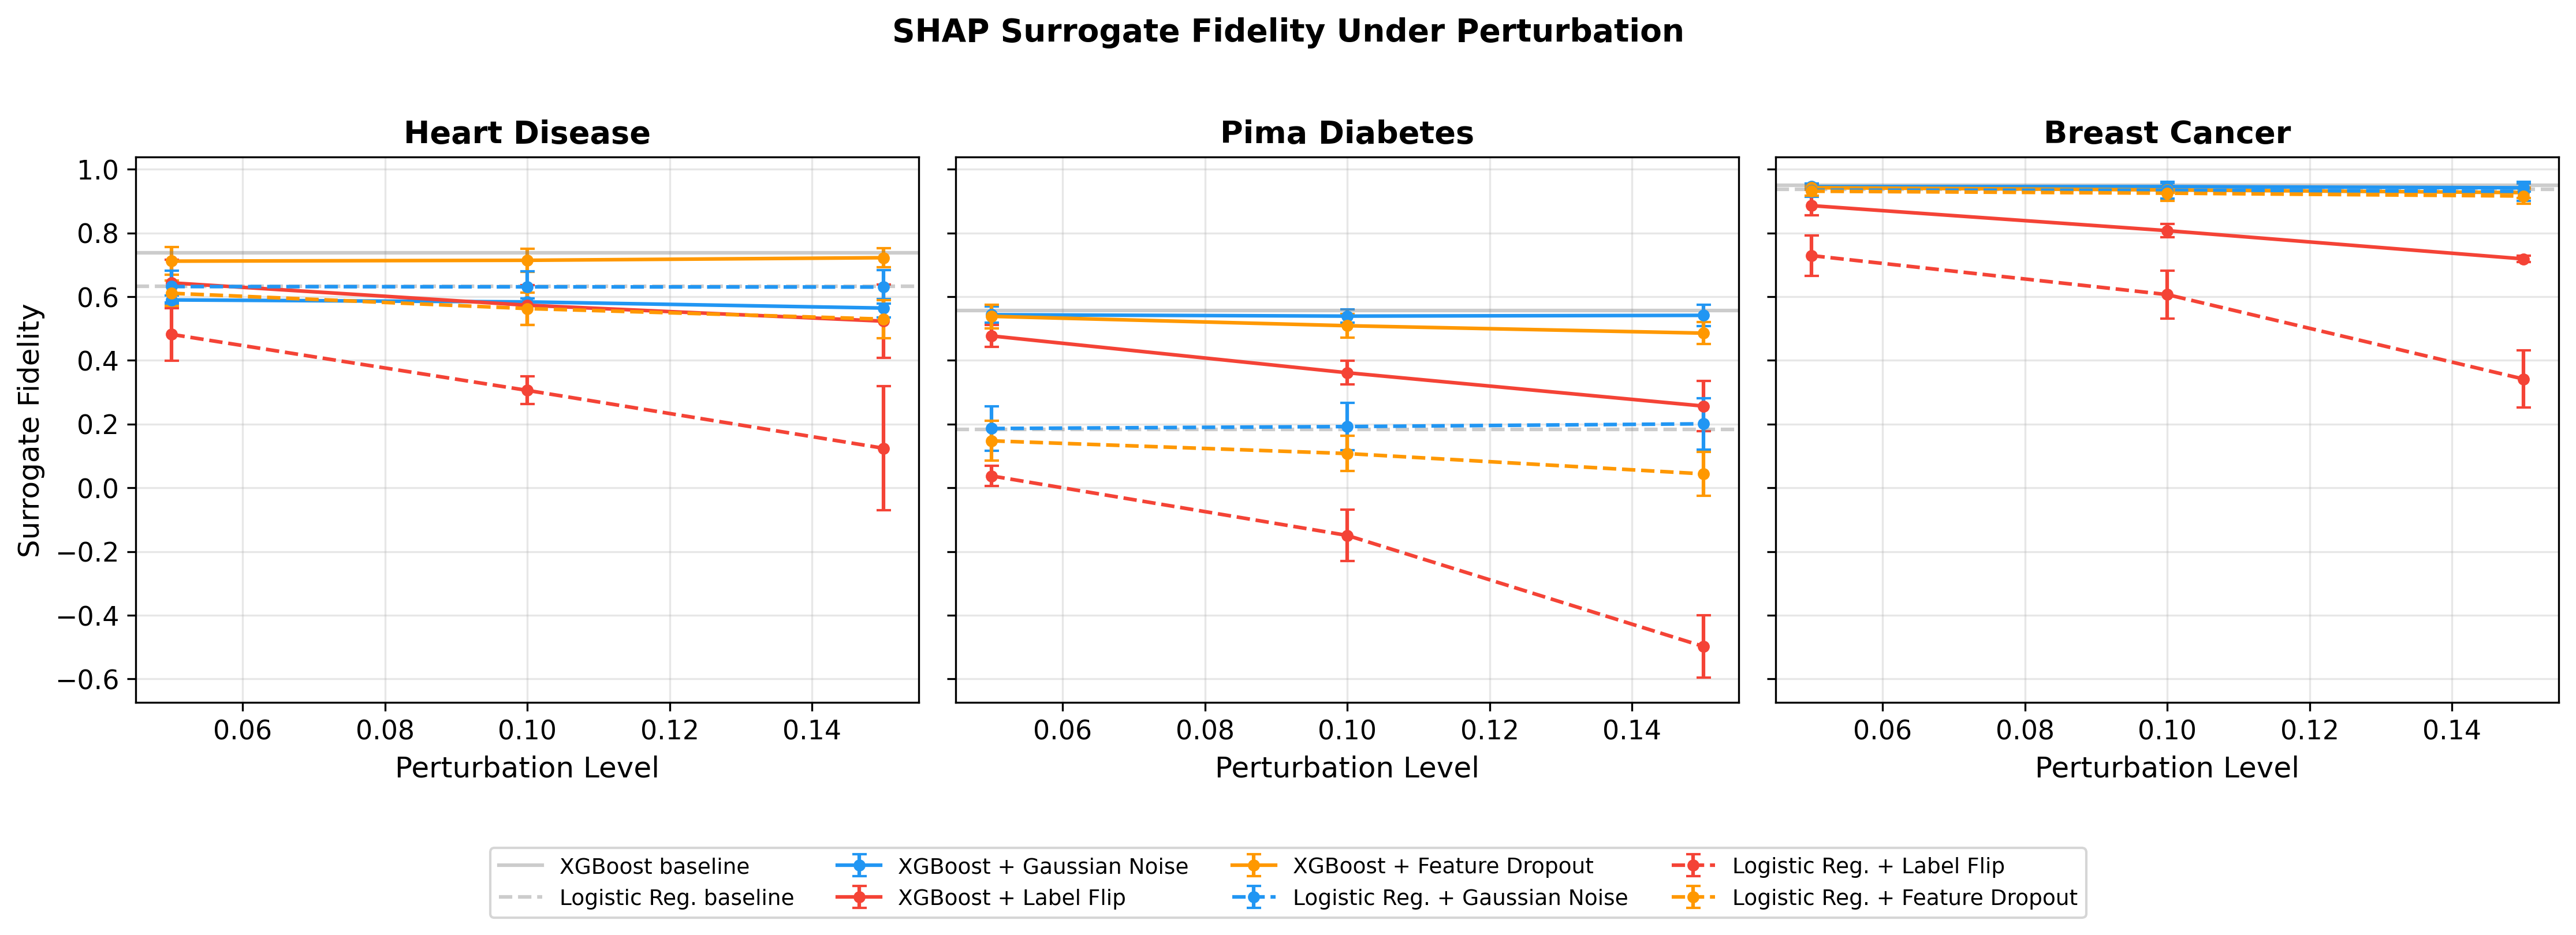
\includegraphics[width=\linewidth]{faithfulness_degradation.png}
\caption{Surrogate fidelity vs.\ perturbation intensity. Under
  label flip, fidelity can drop below zero (dashed line), indicating
  the explanation is worse than the trivial
  baseline.}\label{fig:fidelity}
\end{figure}

% ═════════════════════════════════════════════════════════════════════
\section{Discussion}\label{sec:discussion}

\subsection{Why Label Flip Is So Much Worse}

The key difference is that Gaussian noise and feature dropout change
the test inputs but leave the model unchanged. Since SHAP's exact
methods (TreeExplainer, LinearExplainer) faithfully reflect the model,
the explanations stay accurate even if the inputs are a bit different.

Label flip, on the other hand, corrupts the training data and forces
the model to be retrained. The decision boundary itself moves. So
the instability is coming from the model, not from the explanation
method. We confirmed this by checking that native feature importances
(from the model directly) and SHAP-based importances correlate at
$r \approx 0.99$, meaning SHAP is faithfully reporting what the
model thinks---it is the model that has changed.

\begin{figure}[t]
\centering
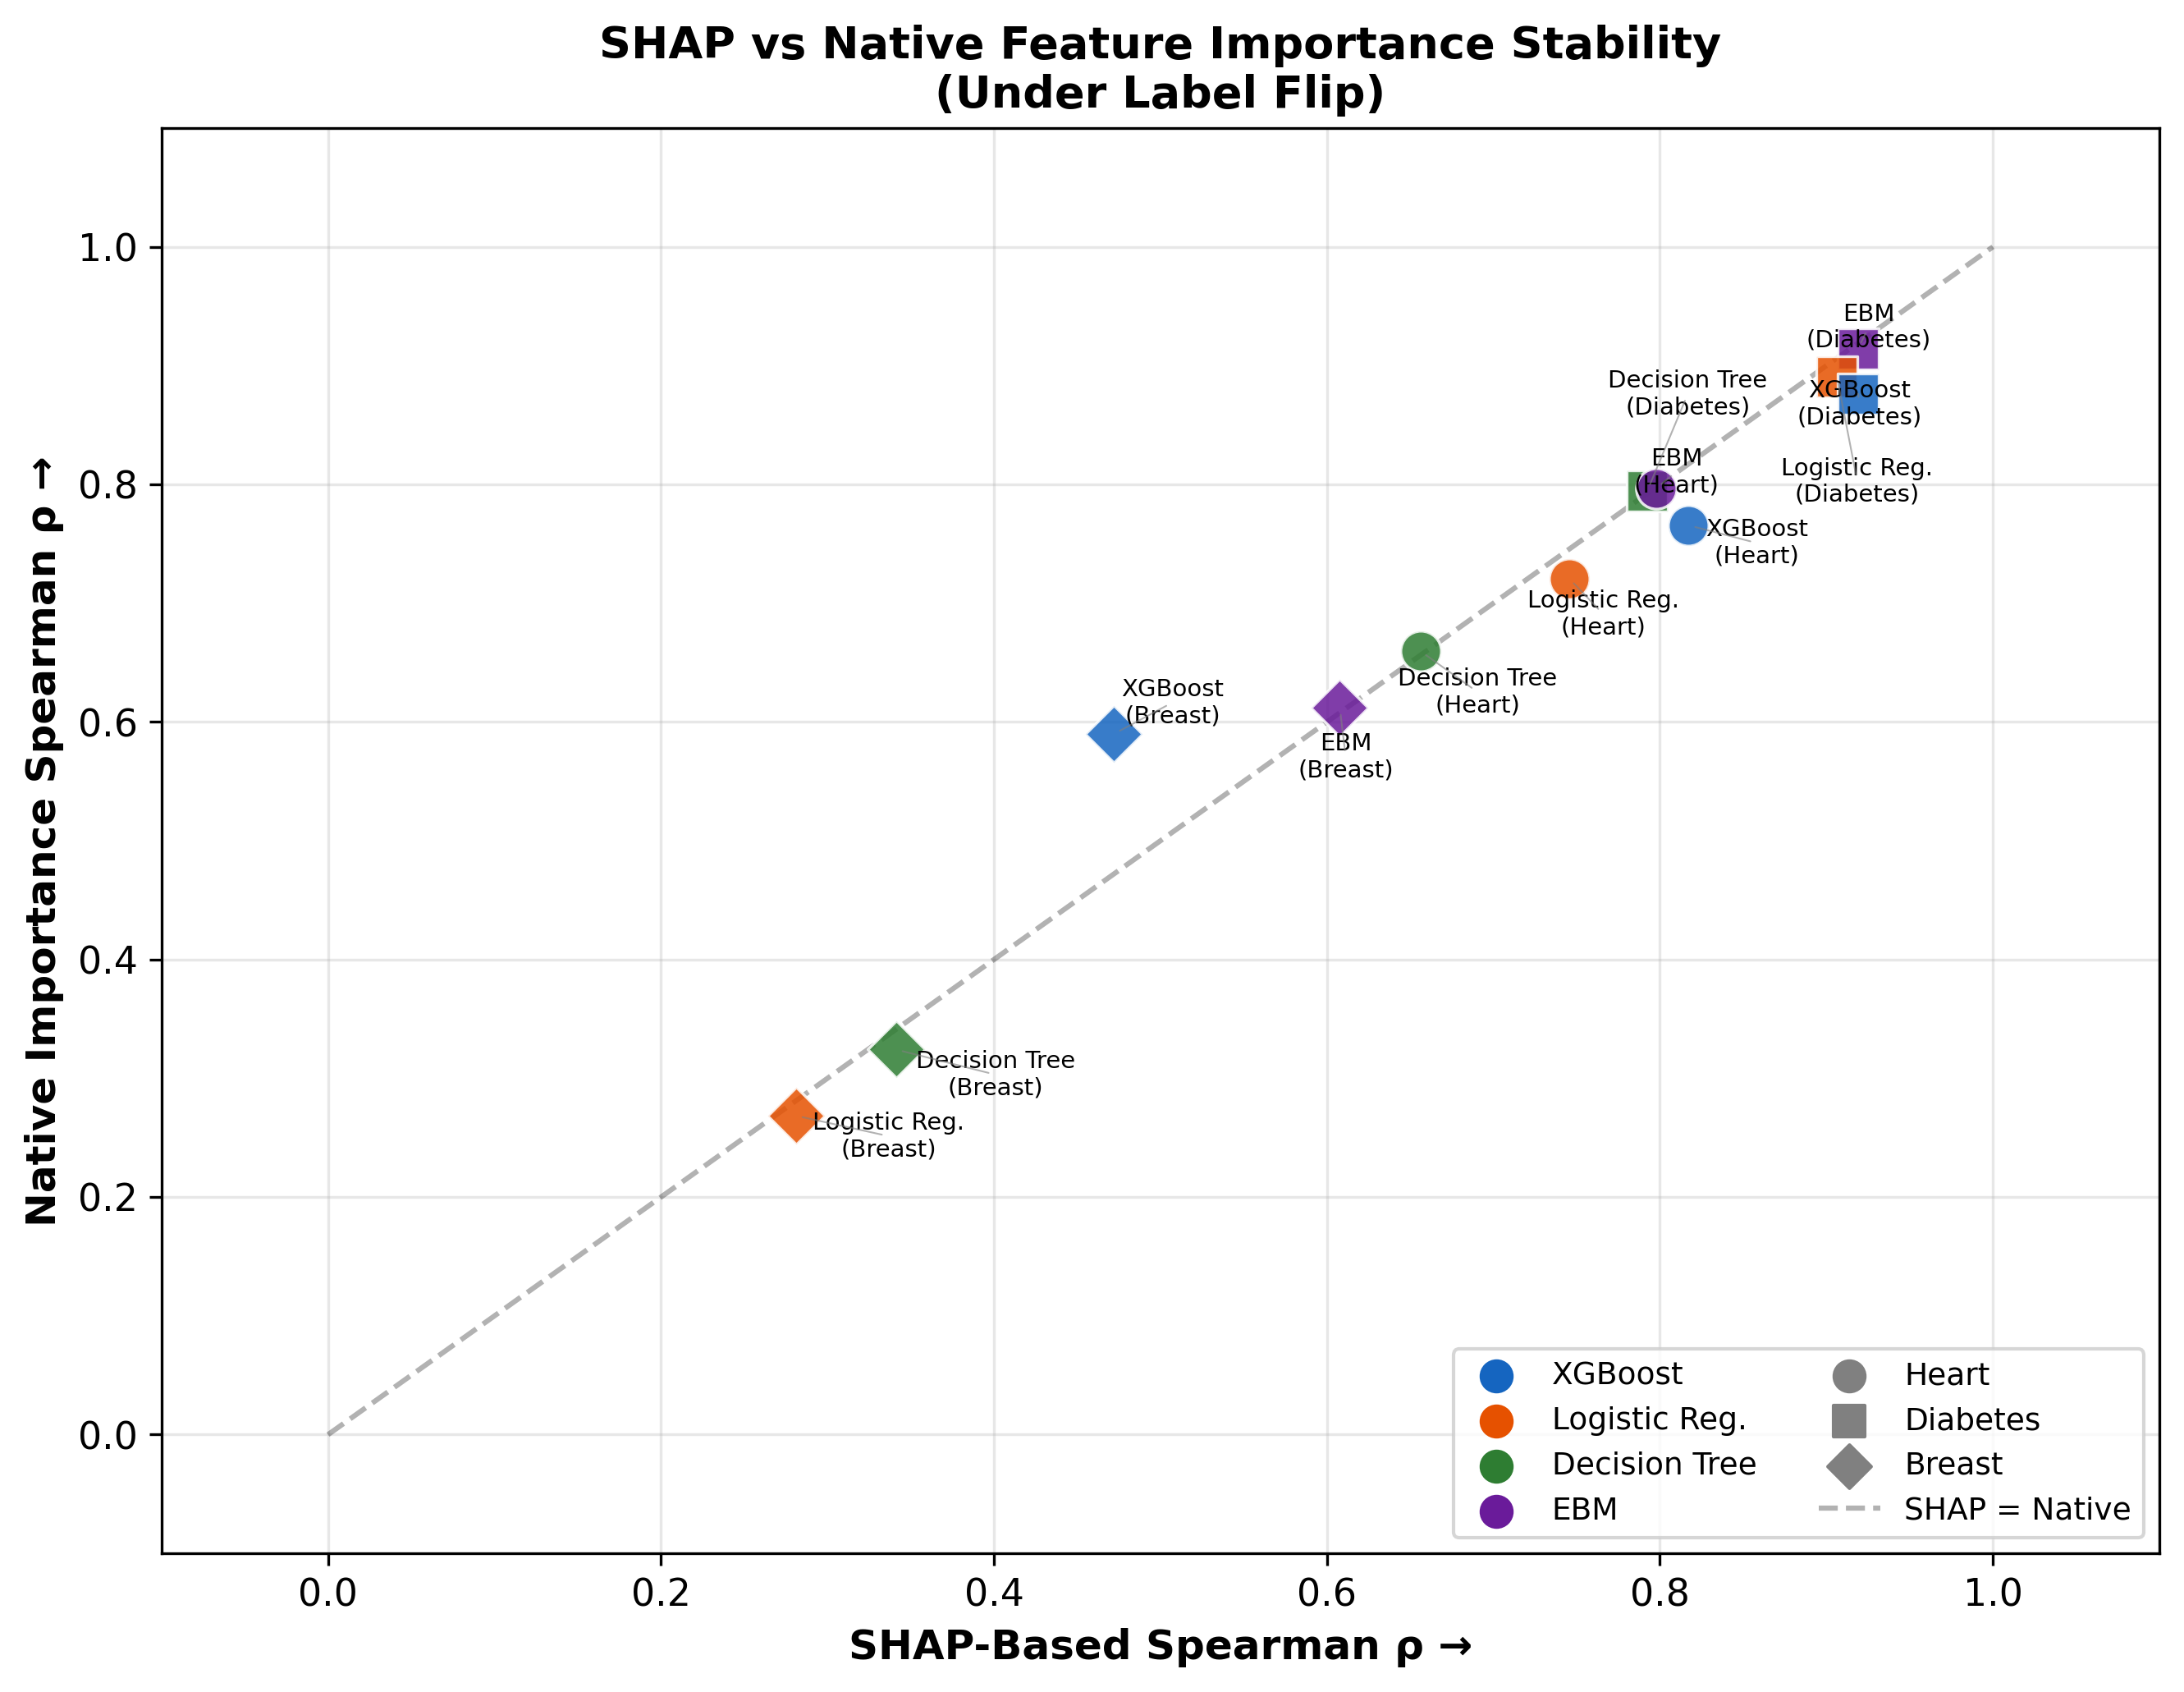
\includegraphics[width=0.9\linewidth]{native_vs_shap.png}
\caption{Native feature importance vs.\ SHAP stability under label
  flip. The tight diagonal clustering confirms that SHAP is
  faithfully reflecting model-level instability.}\label{fig:native}
\end{figure}

\subsection{The Most Important Features Are the Most Fragile}

When we looked at individual features, we found that the ones with
the highest SHAP values (Glucose for Diabetes, worst area for
Breast Cancer, ca for Heart Disease) are also the ones whose
explanations shift the most under label corruption
(Figure~\ref{fig:perfeature}). This is inconvenient: the features
you would rely on most for decision-making are the ones whose
stability you can trust least.

\begin{figure}[t]
\centering
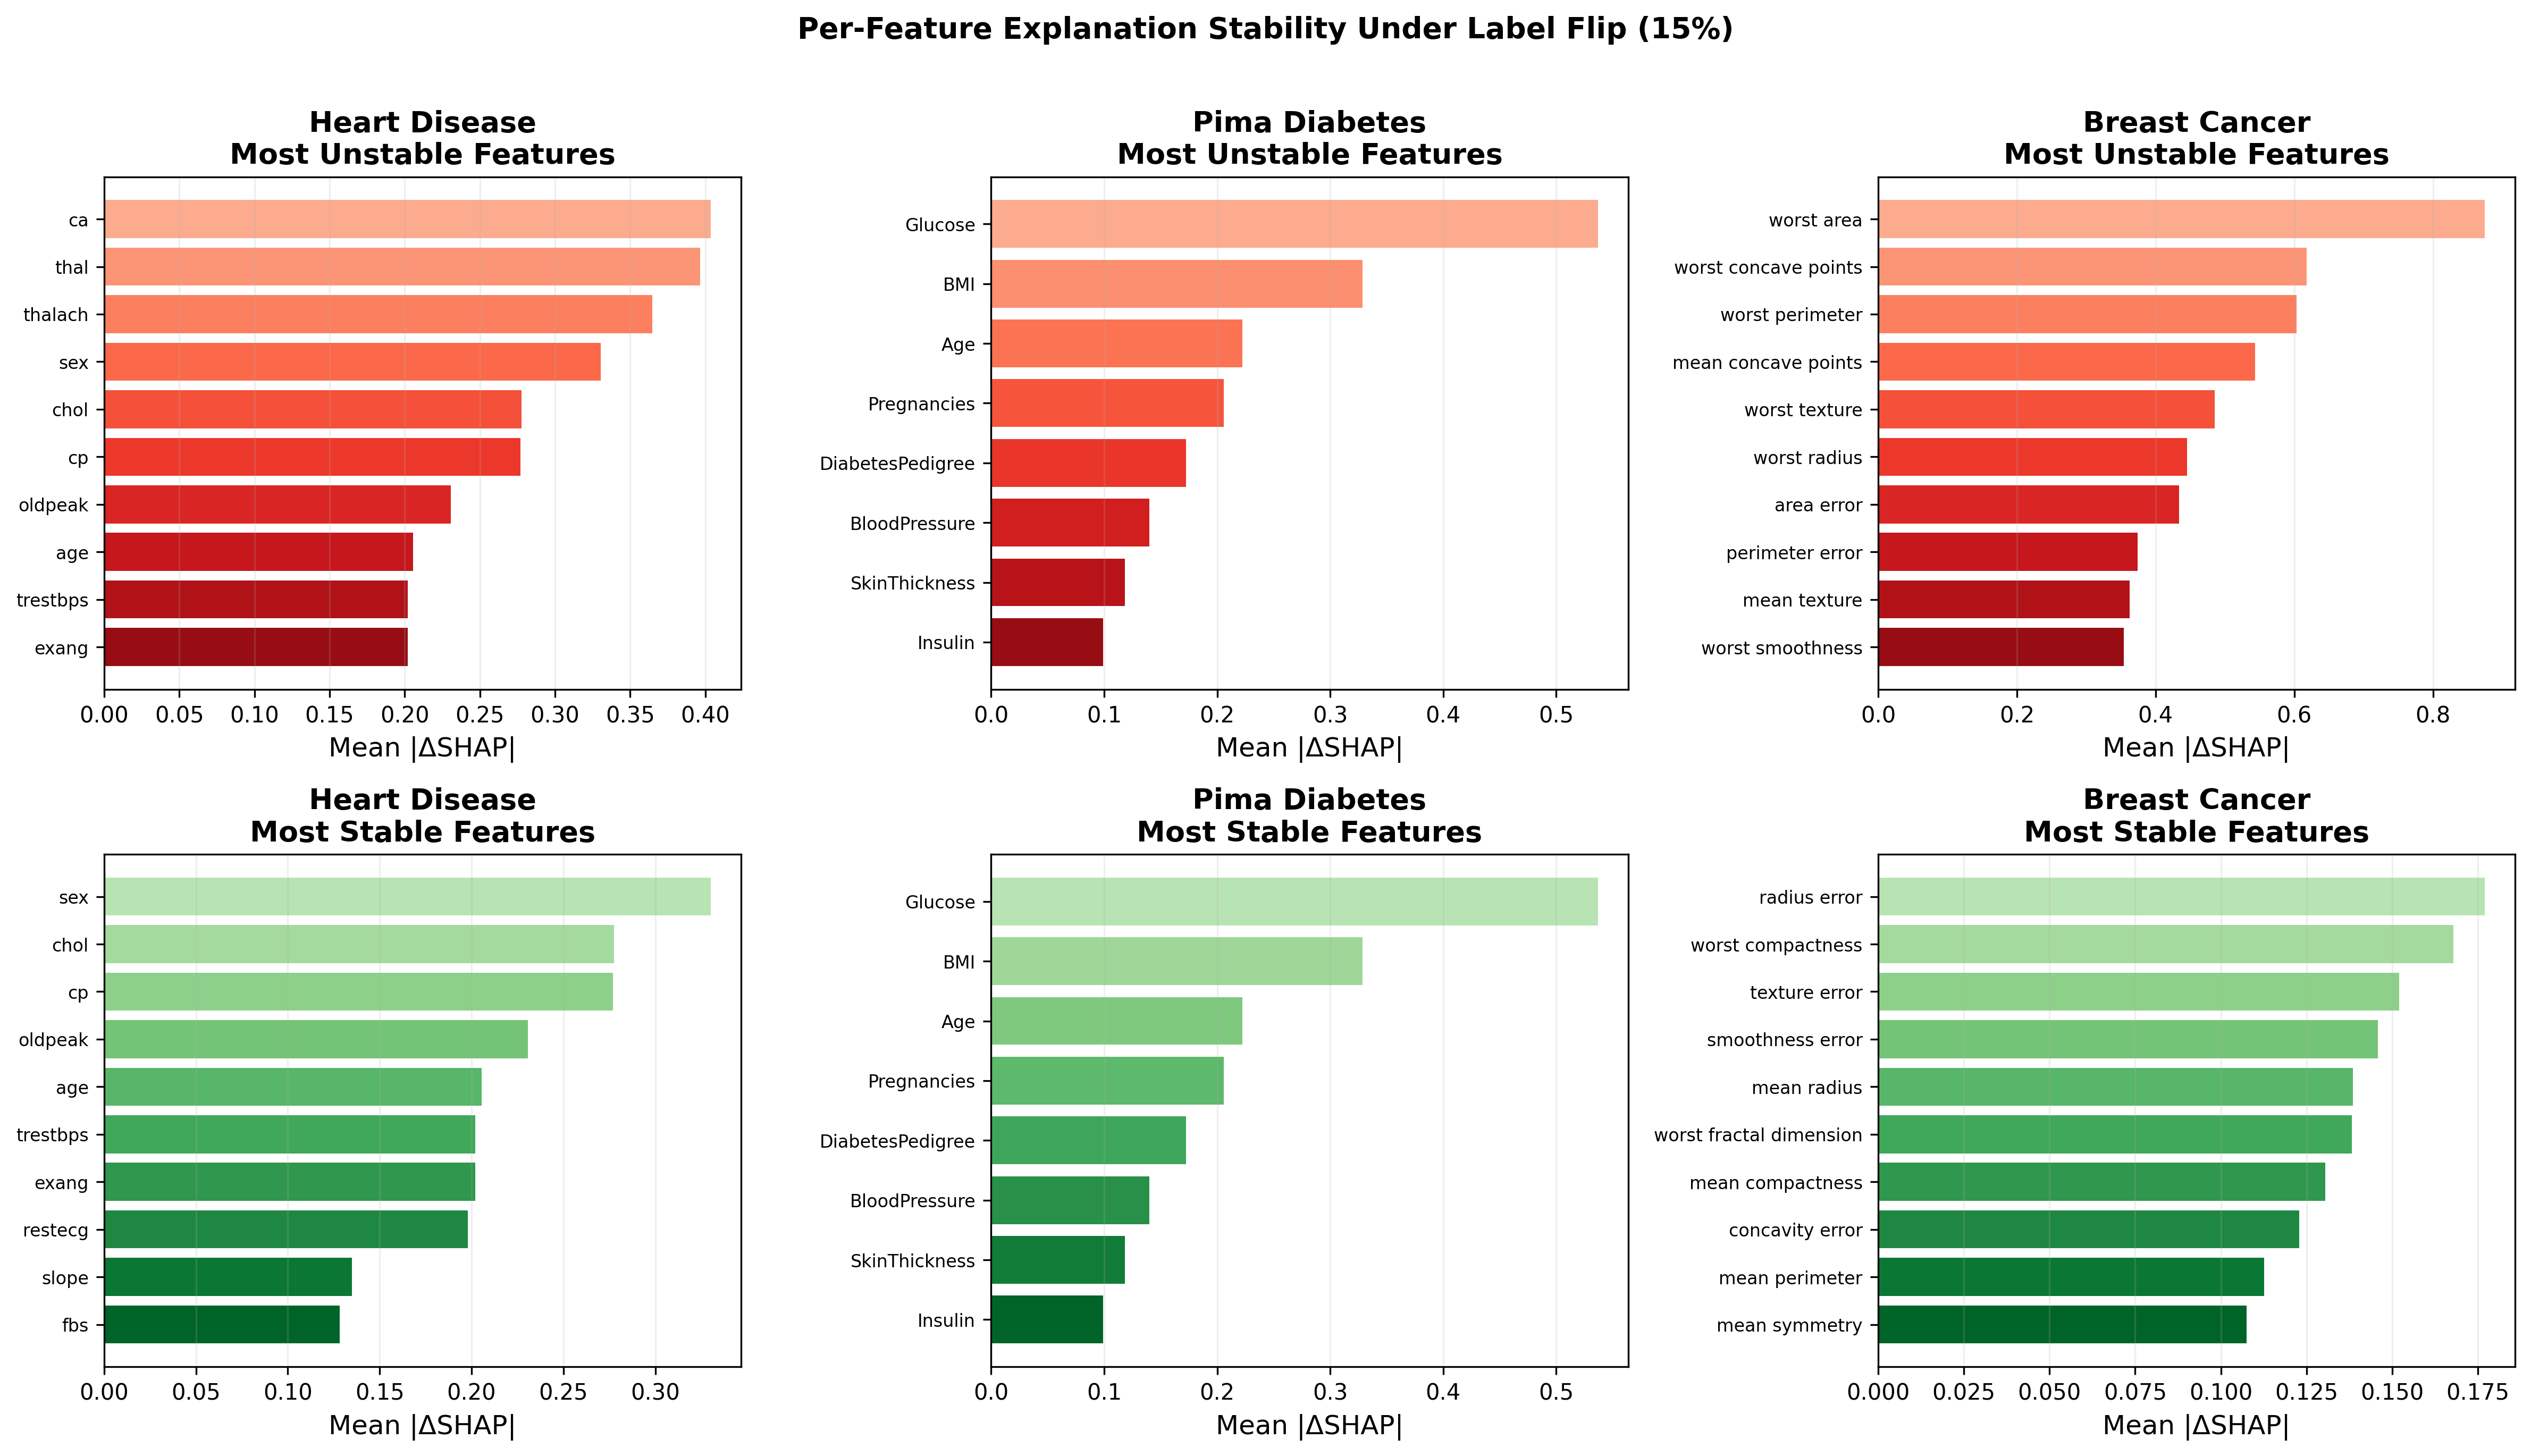
\includegraphics[width=\linewidth]{per_feature_stability.png}
\caption{Per-feature stability under 15\% label flip. Red bars are
  the most unstable features; green bars are the most stable.
  The clinically important features tend to be
  red.}\label{fig:perfeature}
\end{figure}

\subsection{Accuracy vs.\ Stability: A Trade-Off}

Figure~\ref{fig:pareto} shows the accuracy--stability Pareto
frontier. No single model dominates on both axes across all datasets.
For example, Logistic Regression on Breast Cancer gets 98.1\%
accuracy but the worst stability ($\rho = 0.28$). EBM consistently
sits on or near the frontier, making it a reasonable default choice
if you care about both.

\begin{figure}[t]
\centering
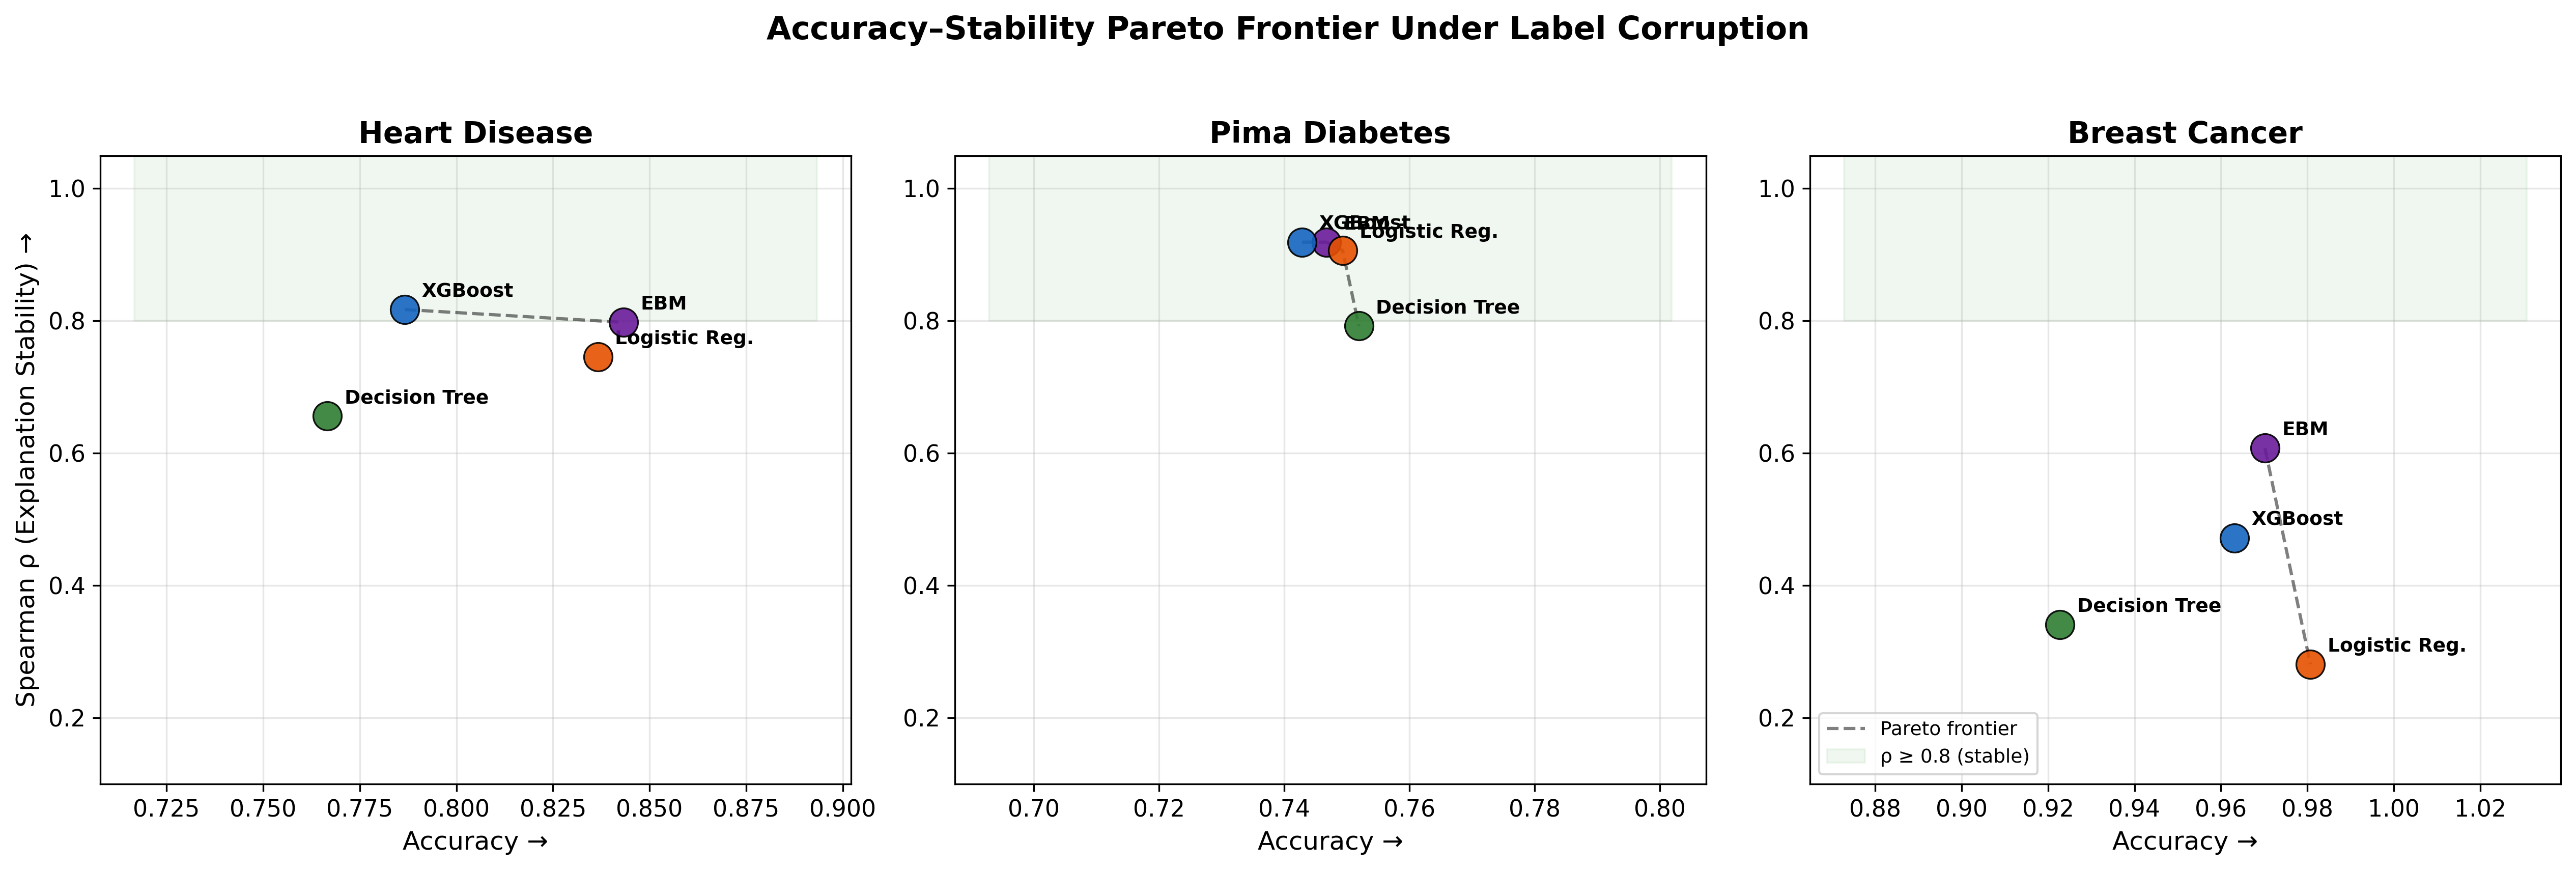
\includegraphics[width=\linewidth]{pareto_frontier.png}
\caption{Accuracy vs.\ stability Pareto frontier under label
  corruption. EBM (green) tends to be on or near the
  frontier.}\label{fig:pareto}
\end{figure}

\subsection{Practical Recommendations}

Based on what we observed:
\begin{enumerate}[leftmargin=*,topsep=2pt,itemsep=1pt]
  \item \textbf{Test stability before deploying explanations.} A
    model can have high accuracy and completely unreliable
    explanations. Checking $\rho$ under simulated label noise is
    a simple sanity check.
  \item \textbf{If you need an interpretable model, consider EBM
    over Decision Trees.} EBM's additive structure seems to give
    it a stability advantage that plain trees do not have.
  \item \textbf{Report both rank and magnitude stability.}
    Spearman $\rho$ alone can hide large shifts in SHAP values.
  \item \textbf{Pay attention to label quality.} In our experiments,
    5\% label corruption causes more damage to explanations than
    15\% Gaussian noise.
  \item \textbf{Check fidelity.} If surrogate fidelity is negative,
    the SHAP explanations are worse than useless and should not be
    the basis for any decision.
\end{enumerate}

\subsection{Limitations}

We want to be upfront about what this study does not cover:
\begin{itemize}[leftmargin=*,topsep=2pt,itemsep=1pt]
  \item We use only 5 random seeds per configuration. This limits
    the statistical power of paired model comparisons (the smallest
    possible Wilcoxon $p$-value with $n=5$ is 0.0625). More seeds
    would strengthen the conclusions.
  \item The three datasets are all small-to-medium tabular
    classification problems. We do not know how well these results
    transfer to large datasets, regression tasks, or non-tabular
    data like images or text.
  \item Our perturbations are synthetic. Real-world distributional
    shift often involves more complex patterns like concept drift or
    covariate shift, which we do not model here.
  \item For EBM, the local explanation is exact for the main additive
    terms, but this breaks down for the pairwise interaction terms
    that EBM also fits. We did not investigate this in detail.
\end{itemize}

% ═════════════════════════════════════════════════════════════════════
\section{Conclusion}\label{sec:conclusion}

We set out to answer a simple question: how stable are SHAP
explanations when the data is noisy? The answer, at least for the
datasets and models we tested, is ``it depends a lot on the type
of noise.''

Gaussian noise and feature dropout barely affect SHAP rankings.
Label corruption, even at low rates, can completely reshape which
features SHAP considers important. Among the four models we tested,
EBM provides the best balance of accuracy and stability, while
Decision Trees---despite their reputation for
transparency---produce the most fragile explanations. Perhaps most
concerning, we found cases where SHAP's fidelity goes negative under
label corruption, meaning the explanation is actively misleading
rather than just noisy.

We think the practical takeaway is straightforward: if you are using
SHAP explanations to make decisions, and there is any chance your
data has label noise, you should test how stable those explanations
are before relying on them. We release the full experimental code
and data to make this easy to reproduce and extend.

\subsection{Future Work}

Several directions seem worth exploring:
\begin{itemize}[leftmargin=*,topsep=2pt,itemsep=1pt]
  \item Extending to temporal distributional shift, where the
    data changes over time (concept drift).
  \item Testing adversarial perturbations designed specifically to
    break explanations.
  \item Scaling up to higher-dimensional data (e.g., genomics,
    NLP embeddings).
  \item Investigating whether training objectives can be modified
    to encourage more stable explanations.
\end{itemize}

% ═════════════════════════════════════════════════════════════════════
% ── Appendix ─────────────────────────────────────────────────────────
\appendix
\section{Additional Figures}\label{app:figures}

\begin{figure}[h]
\centering
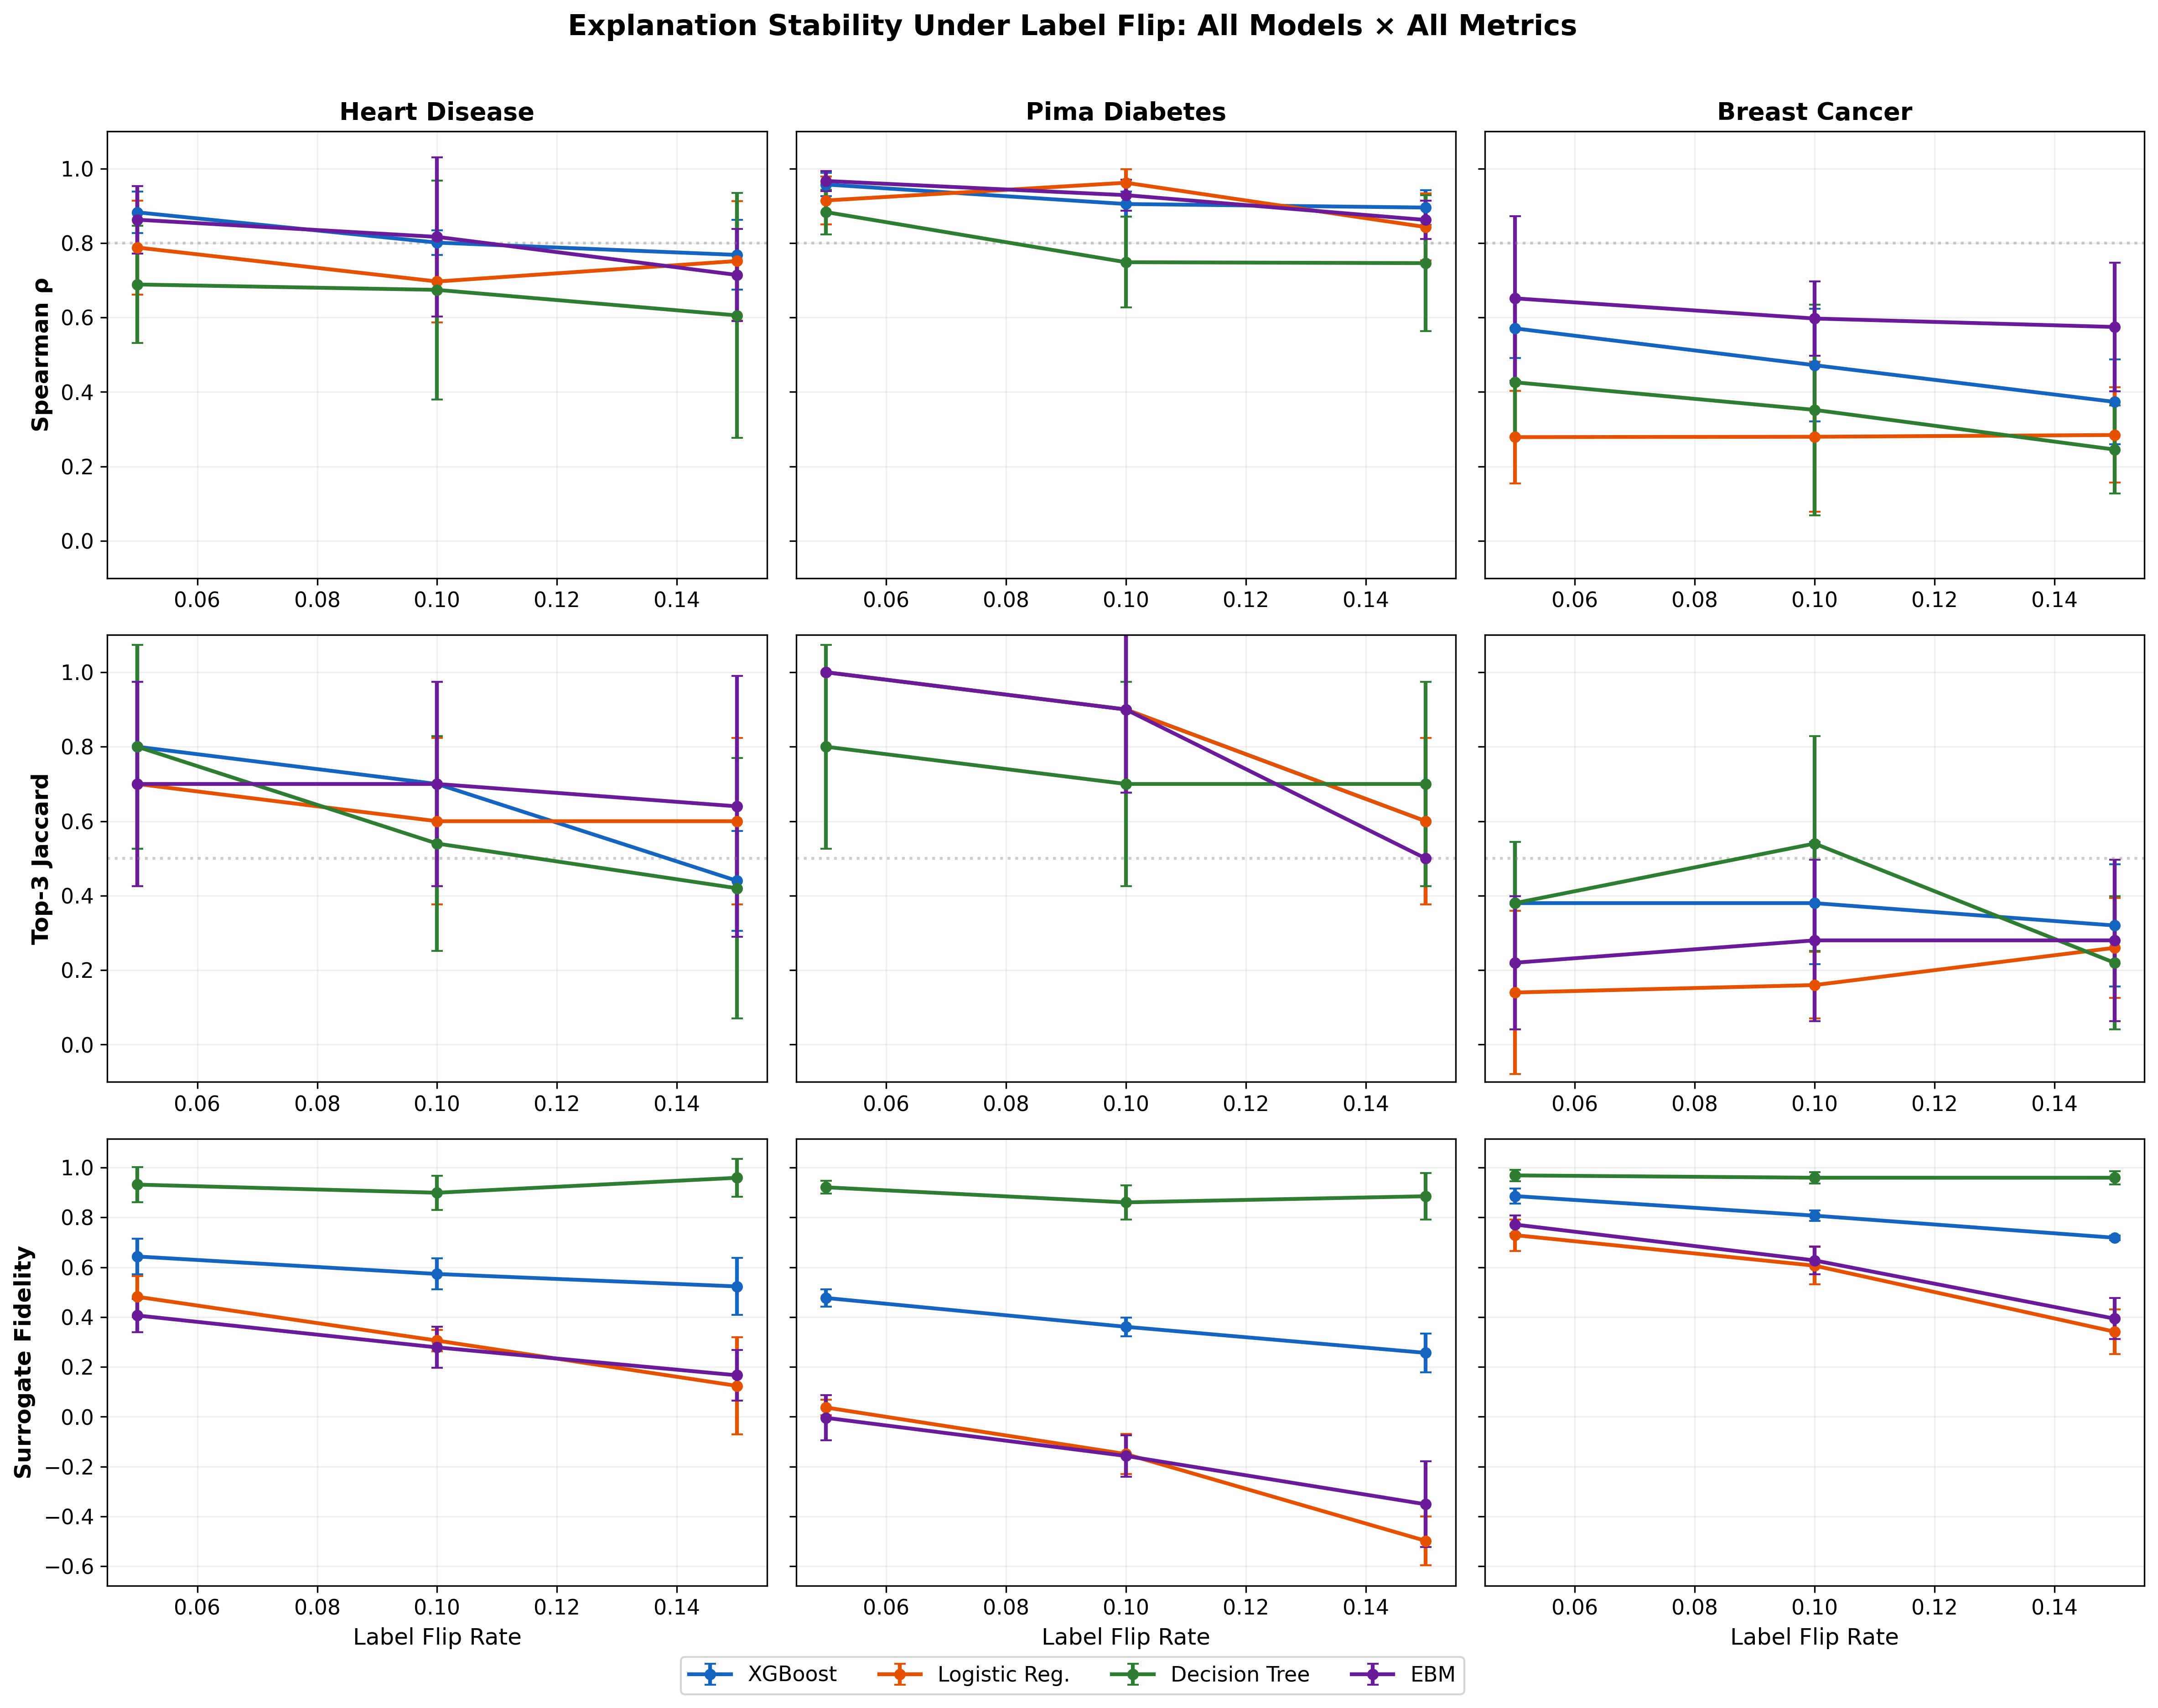
\includegraphics[width=\linewidth]{final_summary_panel.png}
\caption{Summary panel: datasets (columns) vs.\ metrics (rows) under
  label flip for all four models.}\label{fig:summary_panel}
\end{figure}

\begin{figure}[h]
\centering
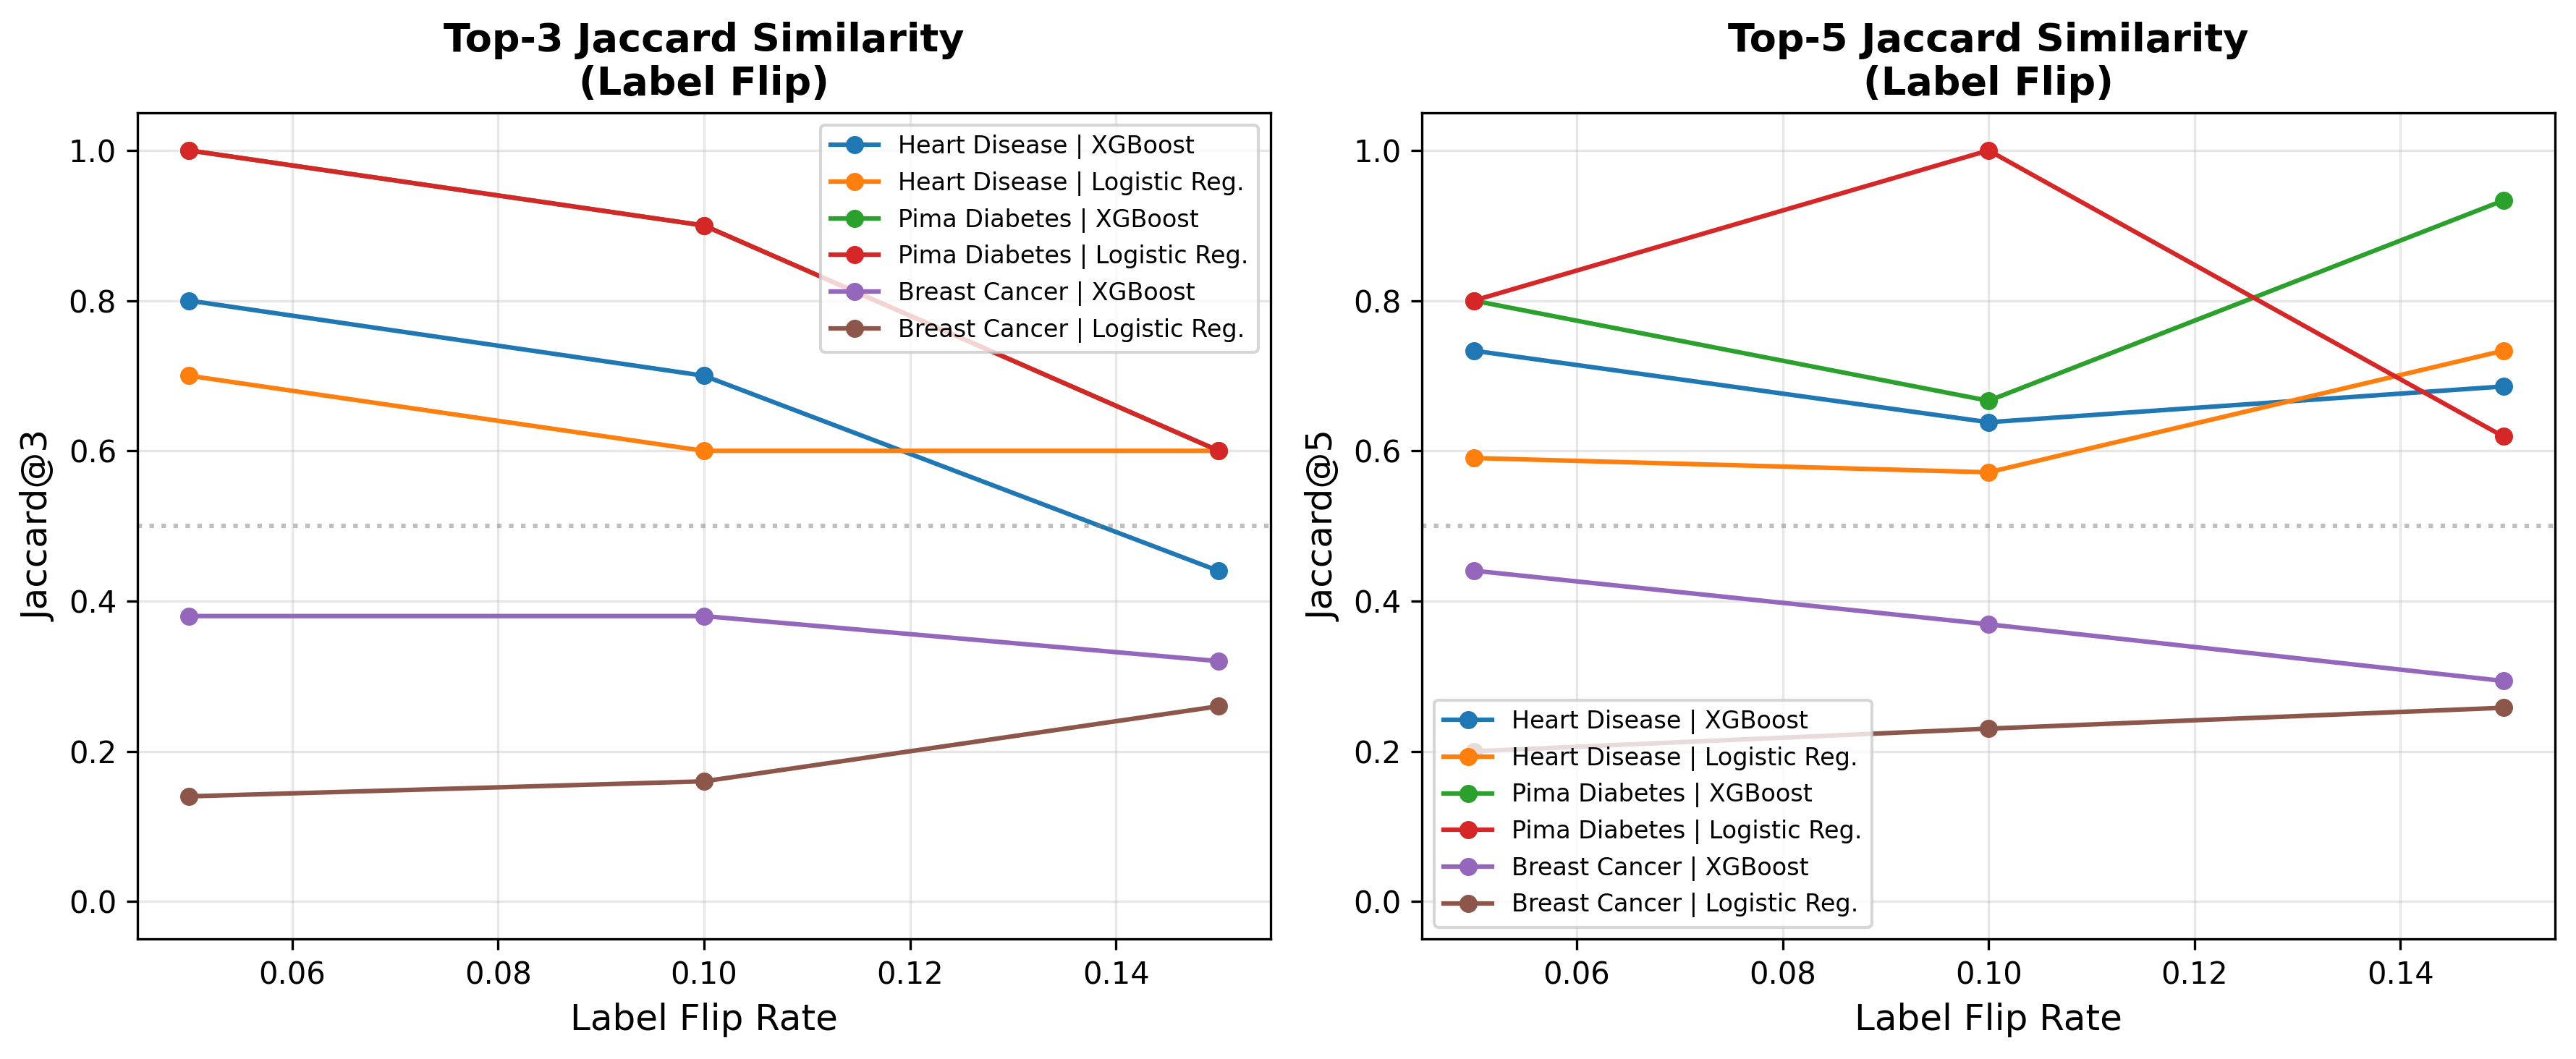
\includegraphics[width=\linewidth]{topk_jaccard.png}
\caption{Top-$k$ Jaccard similarity degradation under label flip
  for $k=3$ (left) and $k=5$ (right).}\label{fig:jaccard}
\end{figure}

\begin{figure}[h]
\centering
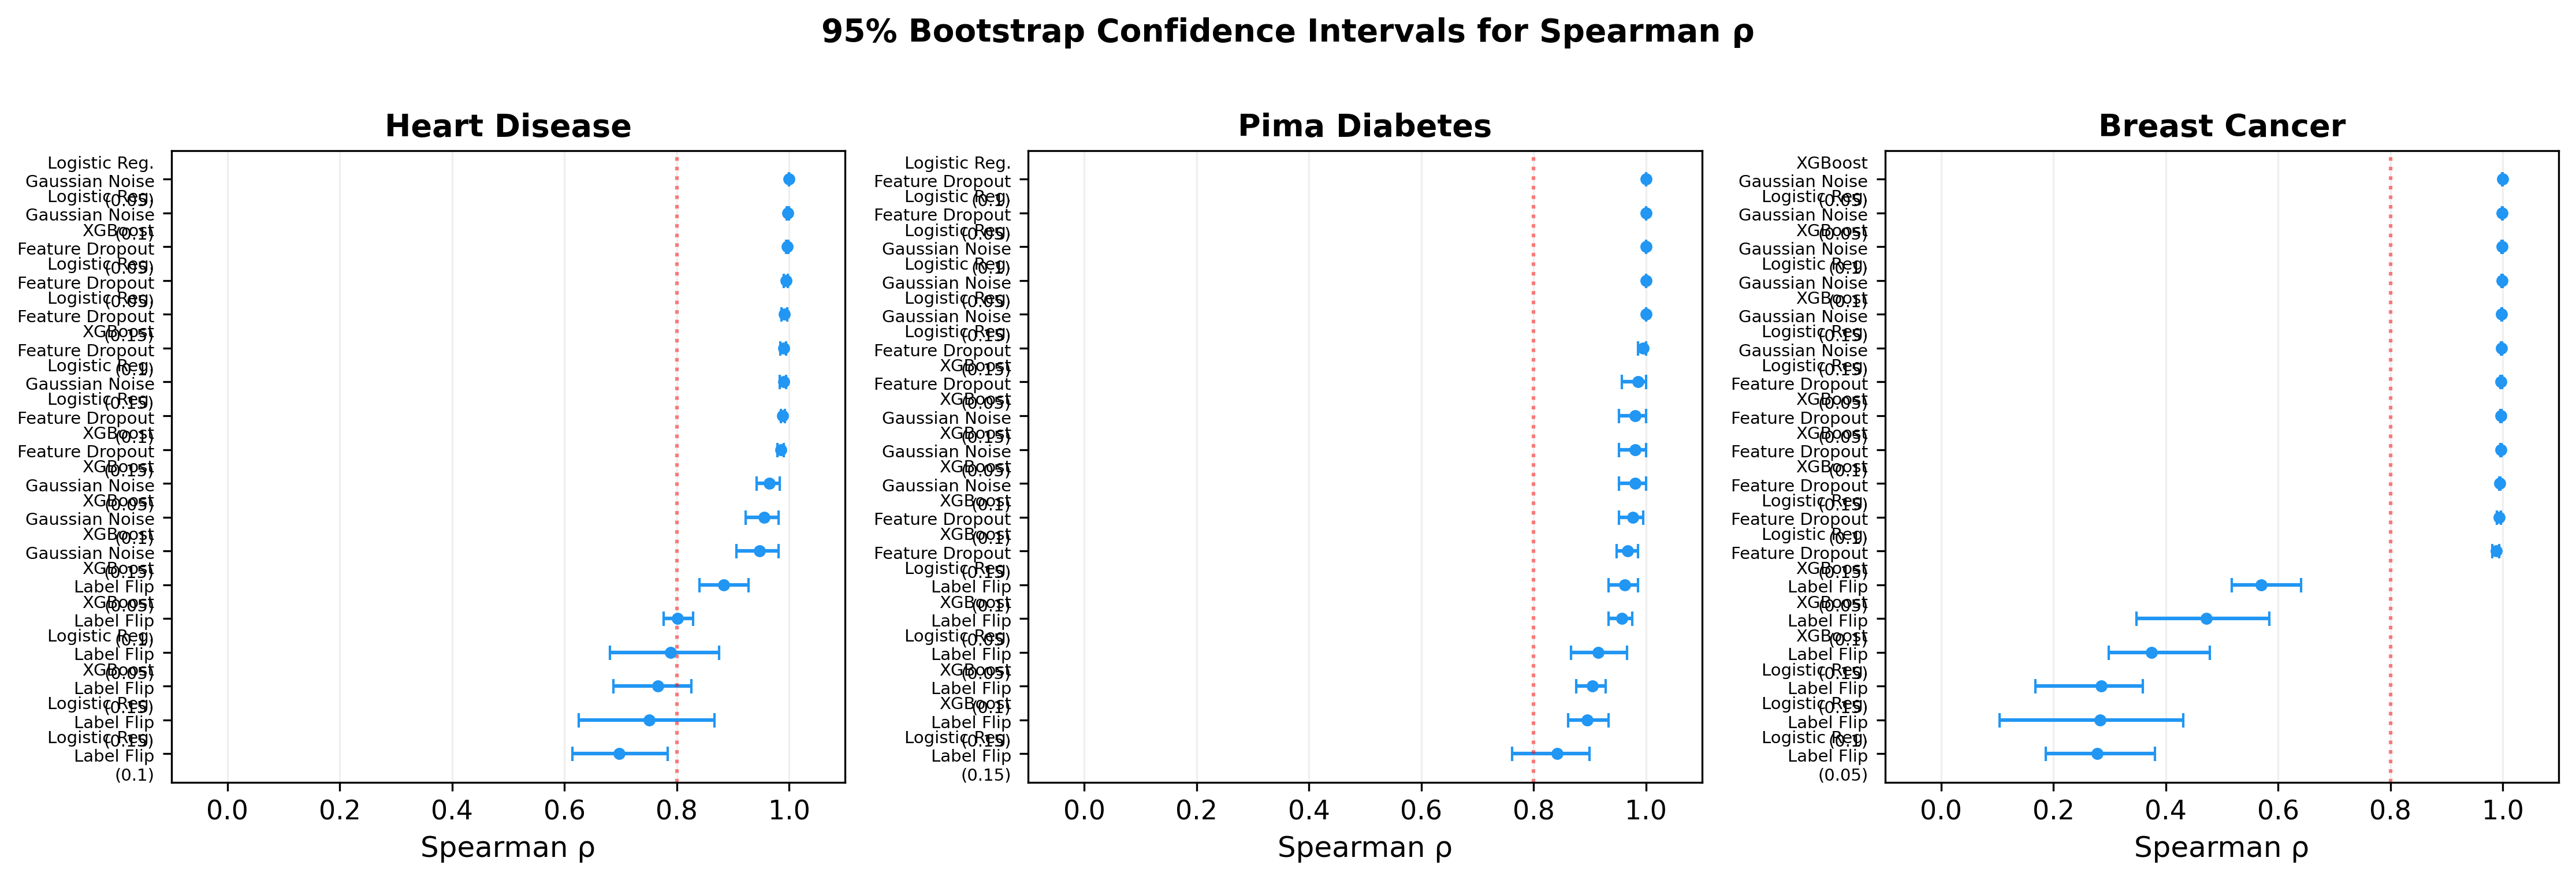
\includegraphics[width=\linewidth]{confidence_intervals.png}
\caption{Bootstrap 95\% confidence intervals for Spearman~$\rho$.
  The label flip intervals are clearly separated from the other
  two perturbation types.}\label{fig:ci}
\end{figure}

\begin{figure}[h]
\centering
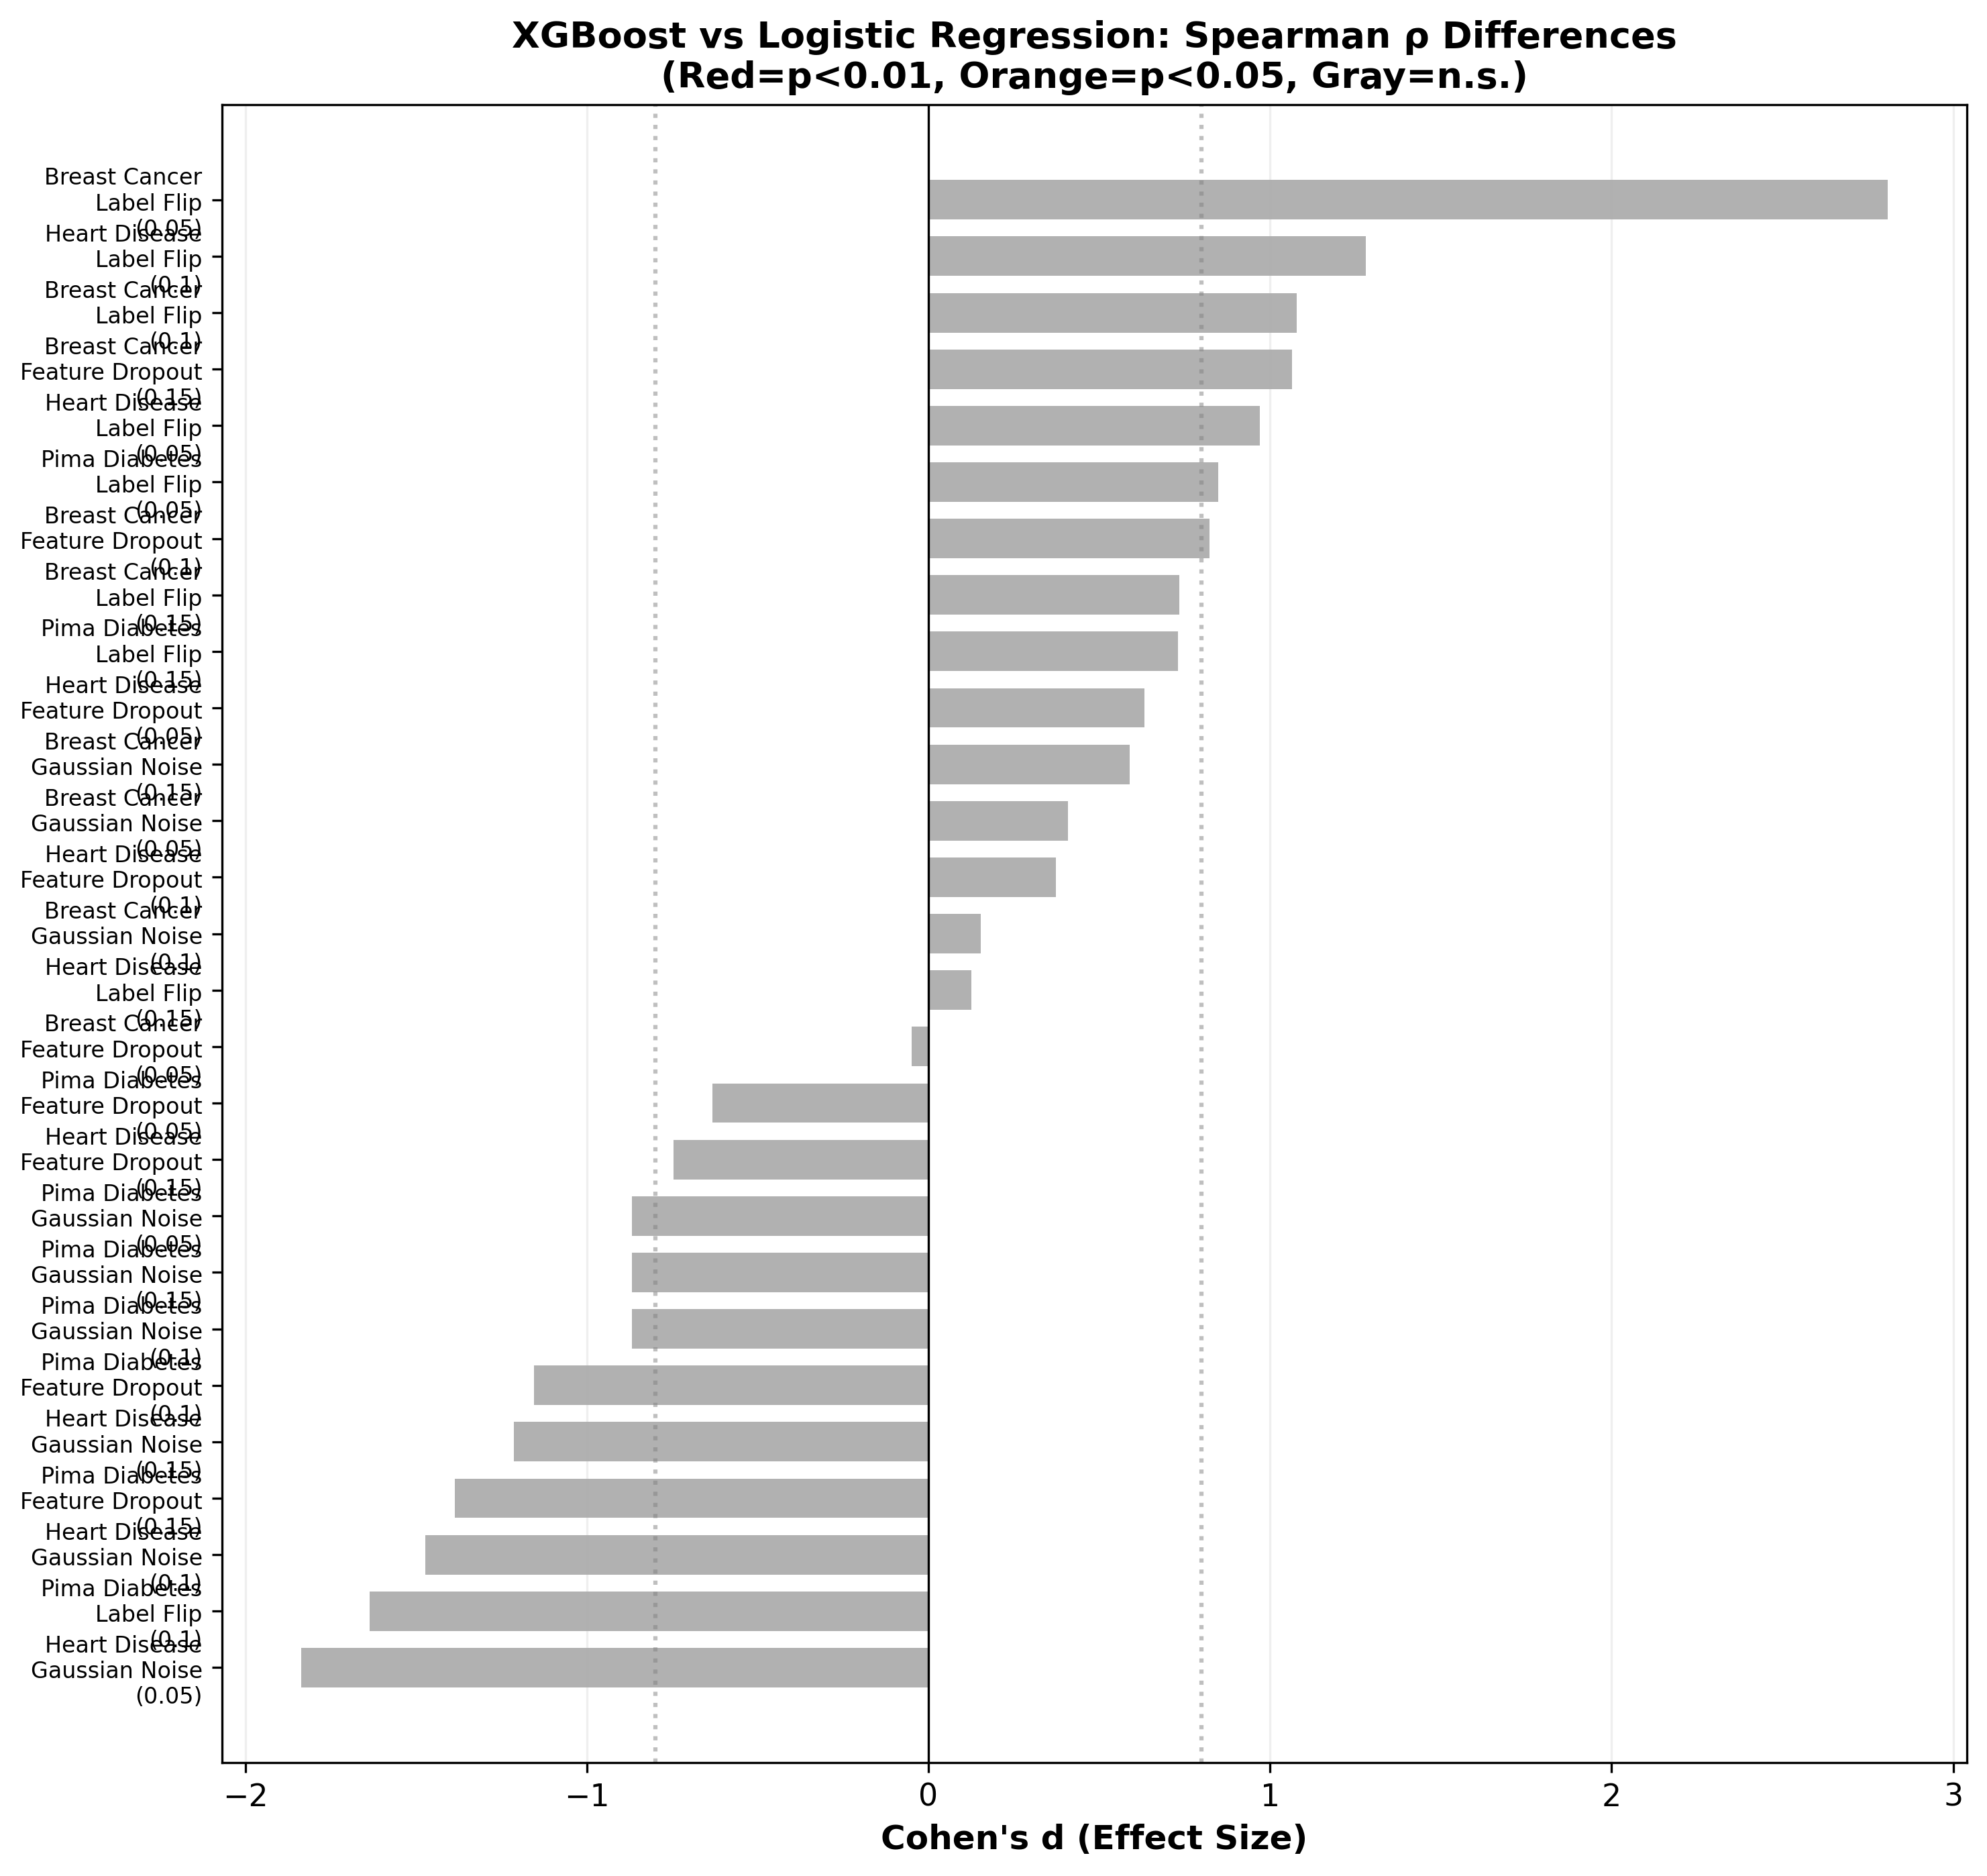
\includegraphics[width=\linewidth]{significance_forest.png}
\caption{Forest plot of Cohen's $d$ effect sizes. Red bars indicate
  $p < 0.01$.}\label{fig:forest}
\end{figure}

\begin{figure}[h]
\centering
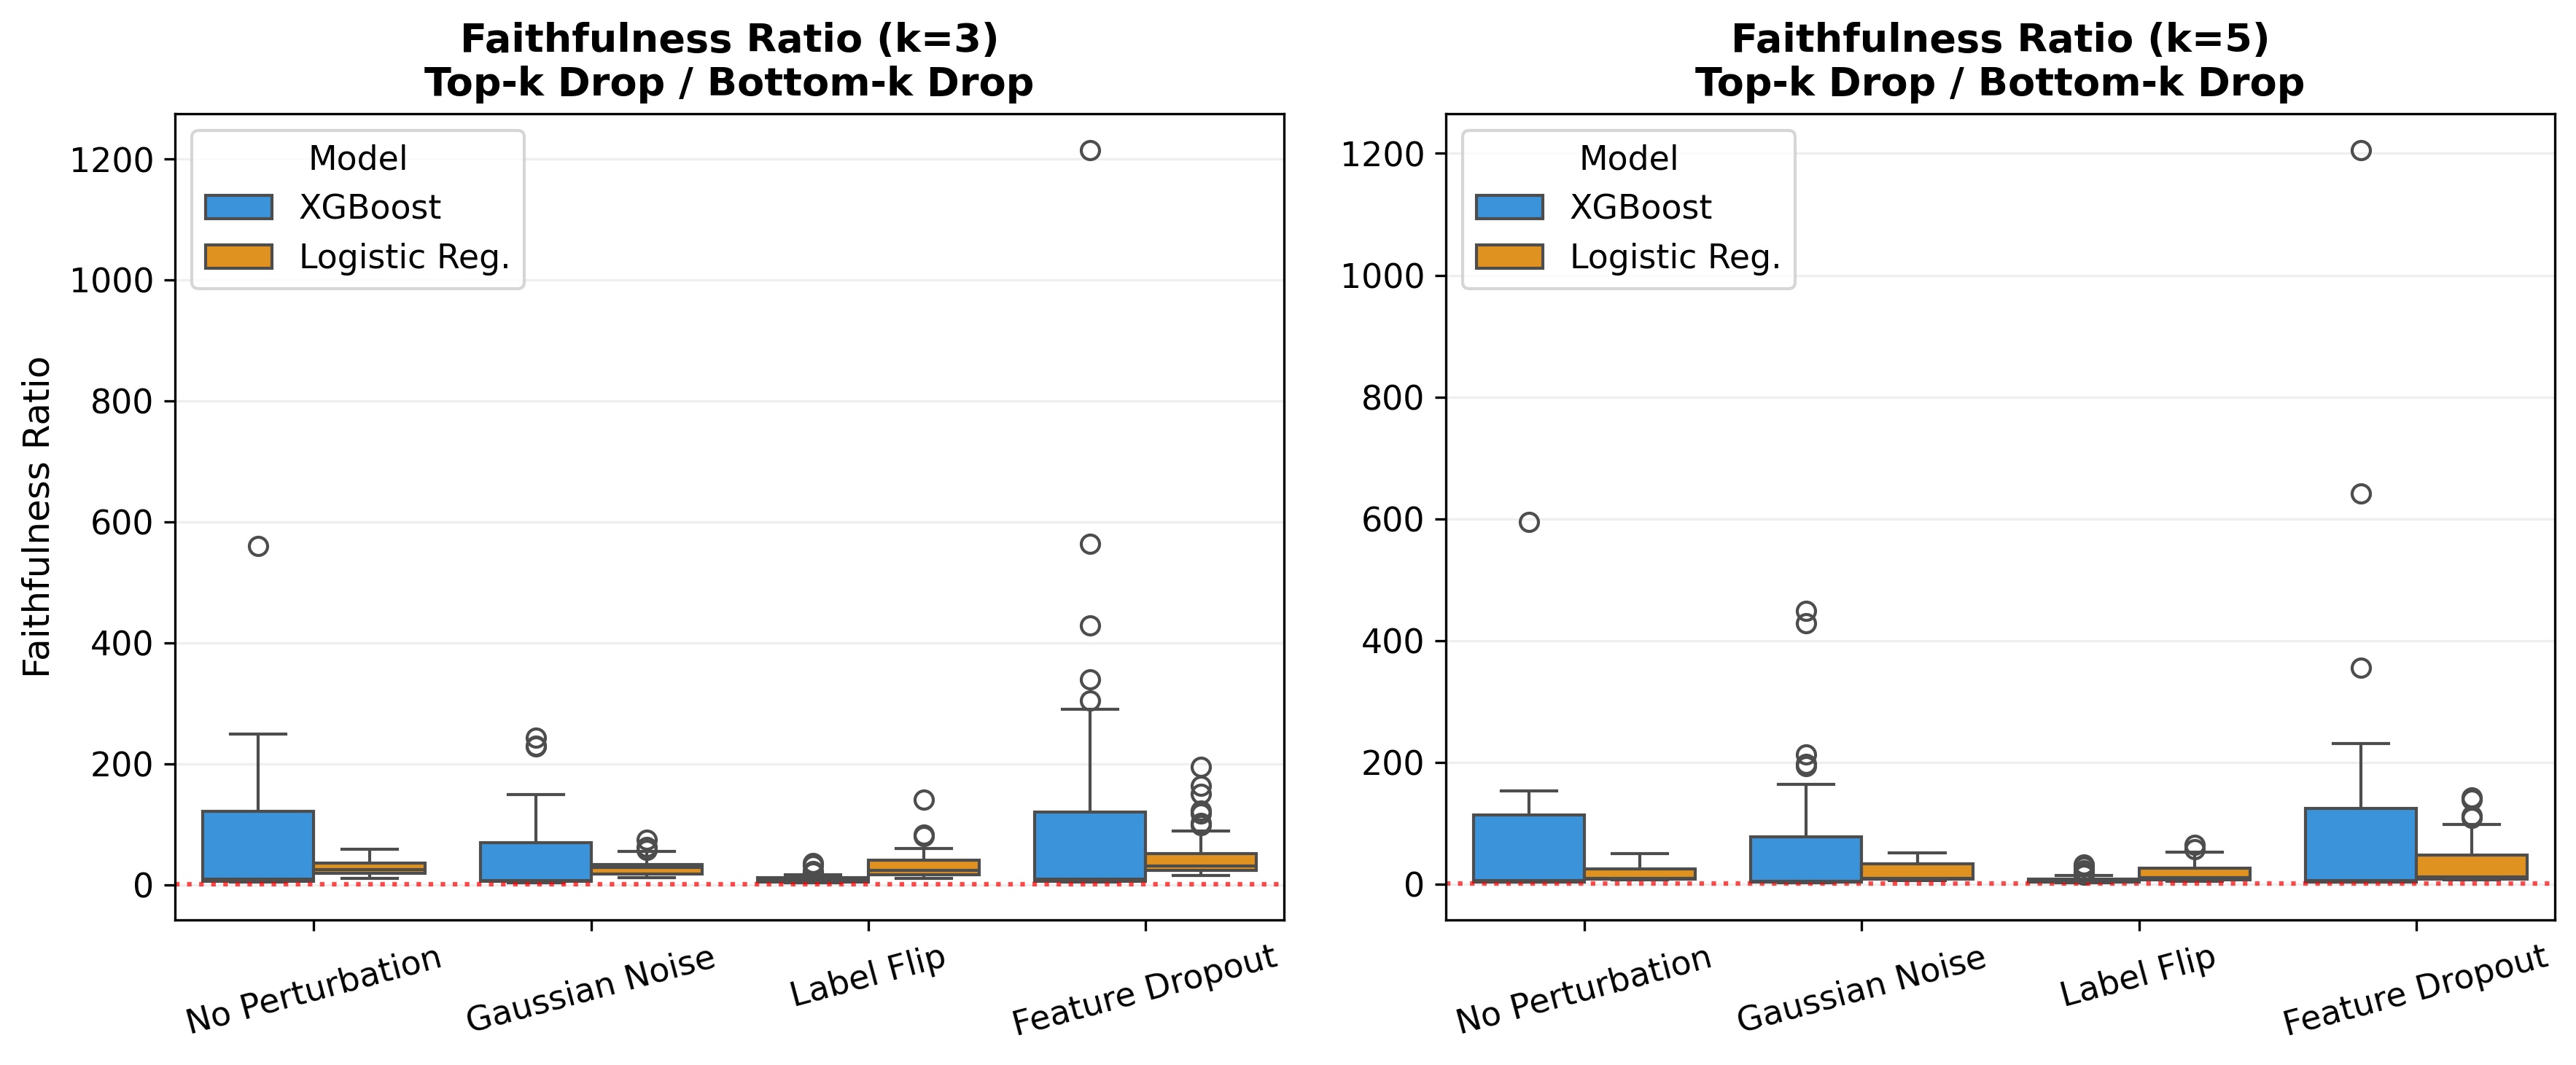
\includegraphics[width=\linewidth]{faithfulness_ratio.png}
\caption{Perturbation faithfulness ratio ($\text{FR}_{k}$). A ratio
  well above 1 means SHAP is identifying the right features. Under
  label flip, the ratios shrink.}\label{fig:fr}
\end{figure}

\begin{figure}[h]
\centering
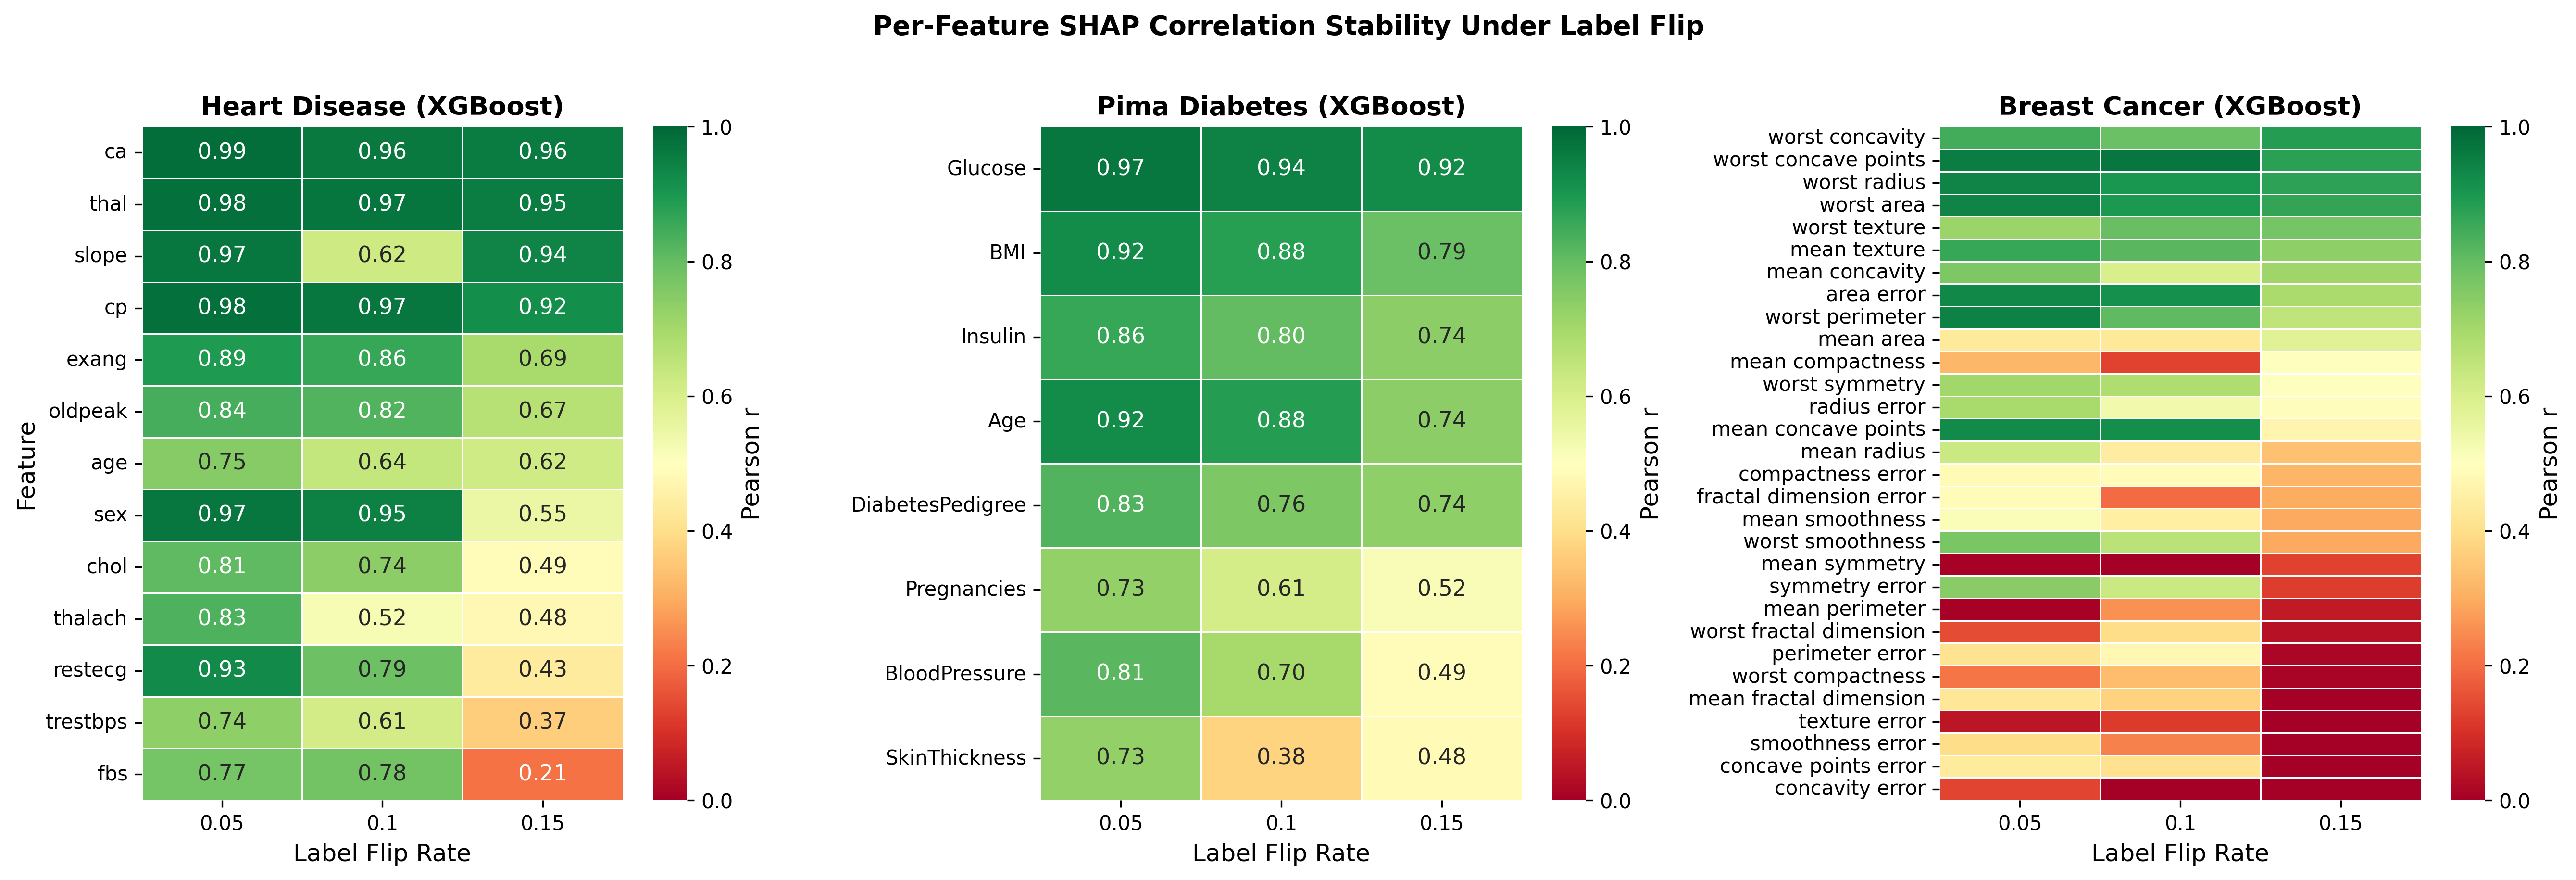
\includegraphics[width=\linewidth]{feature_correlation_heatmap.png}
\caption{Per-feature SHAP correlation under label flip. Individual
  features keep high sample-level correlation, but the aggregate
  ranking across features shifts.}\label{fig:feat_corr}
\end{figure}

% ═════════════════════════════════════════════════════════════════════
% ── Bibliography ─────────────────────────────────────────────────────
\bibliographystyle{plainnat}
\bibliography{references}

\end{document}
